\documentclass[twocolumn]{scrartcl}
%\documentclass[twocolumn,12pt]{article}
%\documentclass{scrartcl}

\usepackage[utf8]{inputenc}
\usepackage[T1]{fontenc}
\usepackage{lmodern}
%\usepackage[ngerman]{babel}
\usepackage[main=ngerman]{babel}
\usepackage{amsmath}

%\usepackage{makeidx}
%\makeindex

\usepackage{fancyvrb}
\usepackage{fvextra}
\usepackage[final]{microtype}

% \usepackage{palatino}
%
% \usepackage{newpxtext,newpxmath}
%
%\usepackage[sc]{mathpazo} % or option osf
\usepackage[osf]{newpxtext}
\usepackage{newpxmath}
\usepackage[output-decimal-marker={,}]{siunitx}

%\usepackage[comma,authoryear]{natbib}
%%\bibliographystyle{natdin}%%\bibliographystyle{apalike}
%\bibliographystyle{apalike-german}

%\usepackage{csquotes}
\usepackage[backend=biber, style=authoryear, natbib=true]{biblatex}
%useprefix=true
\addbibresource{literatur.bib}

\usepackage{adjustbox}
\usepackage[a4paper, margin=1mm, includefoot, footskip=15pt]{geometry}
%\usepackage[a4paper, margin=20mm, includefoot, footskip=15pt]{geometry}
\usepackage{afterpage}

\usepackage{subcaption}
\usepackage[autostyle,german=guillemets]{csquotes}

\usepackage{caption}
\captionsetup{margin=10pt,font=small,labelfont=bf,format=plain,indention=1.em}

\usepackage[pdftitle={Schnellwüchsige, geradschaftige Robinien; Fast-growing, straight-trunked black locust}
, pdfauthor={Georg Kindermann}
, pdfsubject={Waldbau, Waldwachstum, Robinie, geradschaftig}
, pdfkeywords={Waldbau, Waldwachstum, Wald, Forst, Robinie, geradschaftig}
, pdflang={de-AT-1996}
, hidelinks
, pdfpagemode=None]{hyperref}

%\nonfrenchspacing
\sloppy
%\usepackage{breqn} %%
\usepackage{enumitem}
%\usepackage{rotating}
\usepackage{pdflscape}

\usepackage[capitalize,nameinlink]{cleveref}
\usepackage{booktabs}

\title{Schnellwüchsige, geradschaftige Robinien\\Fast-growing, straight-trunked black locust}
\author{Georg Kindermann}
%\date{23. Juli 2025}

\listfiles
\begin{document}

\twocolumn[
  \begin{@twocolumnfalse}
    \maketitle
    \begin{otherlanguage}{english}
    \begin{abstract}
      \begin{center}
        %\textbf{Fast-growing, straight-trunked black locust}
        Summary
      \end{center}
      The black locust (Robinia) copes relatively well with dry sites. However, many varieties develop trunks of inferior quality and are therefore mostly suitable only as firewood. Since the 1930s at the latest, black locusts have been selectively bred for straight growth, rapid development, and good drought resistance. Today, there are more than ten varieties that possess these traits. However, only a few of them are available in Austria. To gain practical experience and allow a comparative assessment of the new varieties, a small-scale trial was conducted in which three varieties purchased in Austria and five in Hungary were planted at three different sites in Austria.
    \end{abstract}
    \end{otherlanguage}
    \begin{abstract}
      \begin{center}
        Zusammenfassung
      \end{center}
      Die Robinie ist sehr tolerant gegenüber trockenen Standorten.
      Viele Sorten entwickeln jedoch einen Stamm von minderer Qualität und eignen sich daher meist nur als Brennholz.
      Spätestens seit den 1930er--Jahren werden Robinien gezielt auf geraden Wuchs, schnelles Wachstum und Trockenresistenz gezüchtet.
      Heute existieren mehr als zehn Sorten, die diese Eigenschaften erfüllen.
      In Österreich sind jedoch nur wenige davon erhältlich.
      Um praktische Erfahrungen zu sammeln und einen vergleichenden Eindruck der neuen Sorten zu ermöglichen, wurden im Rahmen eines Kleinstversuchs drei in Österreich und fünf in Ungarn gekaufte Sorten an drei Standorten
      in Österreich gepflanzt.
    \end{abstract}
  \end{@twocolumnfalse}
]

\tableofcontents

\section{Einleitung}

An Standorten, wo der Niederschlag bereits jetzt limitierend wirkt,
schränken zunehmende
Trockenheit und Wärme sowohl die Bandbreite wirtschaftlich
vertretbarer waldbaulicher Maßnahmen als auch die Auswahl geeigneter
Baumarten zunehmend ein. Unter den heimischen Hauptbaumarten kommen
meist Weiß- (Pinus sylvestris) und Schwarzkiefer (Pinus
nigra) sowie verschiedene Eichenarten in Betracht.
Die heimischen Eichen lassen sich hinsichtlich ihrer Trockenresistenz
meist folgendermaßen reihen:
Stieleiche (Quercus robur), Traubeneiche (Quercus petraea),
Zerreiche (Quercus cerris), Flaumeiche (Quercus pubescens). Leider
nimmt auch die Holzqualität entlang dieser Reihung ab. Das Holz der
Zerreiche kann nicht zur Fassproduktion verwendet werden, da es
aufgrund seiner weiten Poren nicht dicht ist. Zudem ist auch der
Splint breiter.
Flaumeichen mit hoher Stammqualität sind selten. In jüngerer Zeit
wurden jedoch Züchtungen und Kreuzungen mit anderen Eichenarten
entwickelt, die sich durch Genügsamkeit hinsichtlich Niederschlag und eine
gerade Schaftform auszeichnen.

Solange es für einen Standort regionale Baumarten aus tieferen Lagen gibt,
scheint es, angesichts der Klimaerwärmung zweckmäßig, diese in höheren Lagen zu
verwenden. Befindet man sich jedoch in der tiefsten Höhenstufe, tendieren manche
dazu, Baumarten aus südlichen bzw.\ äquatornäheren Regionen zu verwenden.
Dort sind zwar die Temperaturen höher, jedoch unterscheiden sich beispielsweise Sonnenstrahlung und Tageslängen, an die sich Pflanzen, etwa im Hinblick auf den Austriebszeitpunkt angepasst haben könnten \citep{phillips1941tageslaenge} und deren Wachstum beeinflussen \citep{jester1939zuwachsUndTageslaenge}.
Auf demselben Breitengrad findet man höhere
Sommertemperaturen in kontinentaleren Regionen.
%was bei uns in Österreich in Richtung Osten wäre.

Auf Grenzstandorten mit erschwerter natürlicher Verjüngung gewinnen vegetative
gegenüber generativen Verjüngungsformen zunehmend an Bedeutung.
In Hochlagen kommt es bei der Fichte zu Absenkern.
In der Weichholzau bilden Pappel und Weide häufig Wurzelbrut.
Mit zunehmender Trockenheit gestaltet sich die Verjüngung immer
schwieriger, wodurch es zu einer Verschiebung der Betriebsart vom
Hochwald über den Mittelwald hin zum Niederwald kommen kann.
Dieser Wechsel der Betriebsart geht Hand in Hand mit einer Förderung
von Baumarten mit gutem Ausschlagvermögen.
Aus forstwirtschaftlicher Sicht ist
neben Stockausschlag die Fähigkeit zur Bildung von Wurzelbrut auf
verjüngungswidrigen Standorten zu begrüßen, da die Ausschläge nicht an einen
qualitätsmindernden Stock gebunden und daher meist gleichmäßiger auf der Fläche
verteilt sind.

Stockausschlag verliert nach etwa drei Umtrieben deutlich an Zuwachsleistung und
Neuausschlagvermögen.
Deshalb bleibt auch bei vegetativ arbeitenden Bewirtschaftungsformen
die generative Verjüngung über Samen unerlässlich.
Auf den gleichen Zeitraum bezogen, kann im Ausschlagwald sogar
mehr generative Kernverjüngung erforderlich sein als im Hochwald. Geht man davon
aus, dass beide Betriebsarten in der Verjüngungsphase die gleiche
Ausgangsstammzahl benötigen und der Hochwald eine Umtriebszeit von 180~Jahren,
der Niederwald eine von 30~Jahren hat, ergibt sich Folgendes: Wenn der
Niederwald nach drei Umtrieben, also nach 90~Jahren, generativ verjüngt wird,
muss man innerhalb von 180~Jahren beim Hochwald einmal, beim Niederwald hingegen
zweimal generativ verjüngen.
Aus dieser Perspektive würde Niederwald die ohnehin
schwierige Verjüngungssituation sogar verschärfen.
Sein Vorteil liegt jedoch darin, dass bei Ausbleiben einer
erfolgreichen generativen Verjüngung nach der Nutzung die vegetativen
Ausschläge allein den Bestandesschluss wiederherstellen können. Die
generative Verjüngung kann in diesem Fall auf den nächsten oder sogar
übernächsten Hieb nachgeholt werden.

%%% HIER WEITER %%%

Während die Fähigkeit zum Stockausschlag bei den meisten Baumarten mit
zunehmendem Alter deutlich abnimmt, bleibt die Fähigkeit zur
Wurzelbrutbildung, je nach Art, meist lange erhalten. Bei der Robinie
ist eine effektive Verjüngung über Wurzelbrut auch im höheren
Bestandesalter möglich. Im Gegensatz zum Stockausschlag, bei dem der
Neuaustrieb ausschließlich am Stock erfolgt, kann sich Wurzelbrut,
auch in größerer Entfernung vom Stamm, entlang der horizontal
verlaufenden Wurzeln entwickeln. Da bei langen Umtriebszeiten die
Stammzahl des Altbestandes stark abnimmt, wären bei Verjüngung über
Stockausschlag mit langen Umtriebszeiten die Austriebe weit
voneinander entfernt, was den Bestandesschluss deutlich verzögern
würde. Deshalb wird bei Verjüngung über Stockausschlag in der Regel
eine kurze Umtriebszeit gewählt. Bei Verjüngung über Wurzelbrut
hingegen kann selbst bei geringer Stammzahl im Altbestand, eine dichte
und flächige Naturverjüngung erfolgen. Die Robinie eignet sich daher
auch bei langen Umtriebszeiten gut für eine vegetative
Bestandesverjüngung.

Nach dem Hieb wird der Bestandesschluss im Ausschlagwald meist deutlich
schneller wiederhergestellt als im Hochwald. Dies wird mitunter als Hinweis auf
eine höhere Zuwachsleistung des Niederwaldes interpretiert. Dabei wird jedoch
übersehen, dass beim Niederwald die Fläche in deutlich kürzeren Abständen und
damit öfter als beim Hochwald freigestellt wird. Eine höhere Zuwachsleistung des
Niederwaldes im Vergleich zum Hochwald ist daher nicht zu erwarten.

Während beim Stockausschlag die Zuwachsleistung und das Neuausschlagvermögen bei
jedem abermaligen Hieb stetig abnimmt, zeigt Wurzelbrut diesen unerwünschten
Effekt kaum bis gar nicht. Ausreichend Wurzelbrut bilden von den heimischen
Baumarten Aspe (Popukus tremula), Grauerle (Alnus incarna), Ulme (Ulmus spp.),
Feldahorn (Acer campestre), Kirsche (Prunus avium) sowie Wildobst. Von den nicht
heimischen bilden beispielsweise Robinie (Robinia pseudoacacia) oder Götterbaum
(Ailianthus altissima) reichlich Wurzelbrut.

Diese Eigenschaft ist aber auch ein Grund, warum diesen Baumarten das
Potential eines invasiven Neophyten attestiert wird. Sie sind dadurch
eher als andere Baumarten in der Lage, beispielsweise Trockenrasen zu
besiedeln.
Aber auch auf Trockenrasen scheint die Dauerhaftigkeit des
Robinienholzes geschätzt zu werden. Selbst im Nationalpark wird es als
rustikaler Pflock verwendet (Abb.~\ref{fig:feldmannstreu}).
Dabei wird man die Frage
stellen dürfen, wie diese Trockenrasengesellschaften entstanden sind.
Gelegentlich wird sich zeigen, dass sie in der Vergangenheit durch
(Brand\mbox{--)}Rodung eingeleitet wurden, ein Vorgang, der
neuerdings, offenbar in wörtlicher Anlehnung an den englischen Begriff
deforestation, als \enquote{Entwaldung} bezeichnet wird. Danach kam es
zu Erosion, Plaggenwirtschaft und Beweidung, meist durch Schaf und
Ziege. Nach Einstellung der Bewirtschaftung ist eine natürliche
Sukzession, zunächst über heimische Sträucher wie Schlehe (Prunus
spinosa), Weißdorn (Crataegus monogyna), Hundsrose (Rosa canina),
Kreuzdorn (Rhamnus cathartica), Liguster (Ligustrum vulgare),
Berberitze (Berberis vulgaris), Rote Heckenkirsche (Lonicera
xylosteum), Besenginster (Cytisus scoparius), Heidelbeere (Vaccinium
myrtillus), Kornelkirsche (Cornus mas) oder Roter Hartriegel (Cornus
sanguinea) in Richtung eines Waldes mit Traubeneiche (Quercus
petraea), Stieleiche (Quercus robur), Zerreiche (Quercus cerris),
Flaumeiche (Quercus pubescens), Hainbuche (Carpinus betulus),
Feldahorn (Acer campestre), Birke (Betula pendula), Weißkiefer (Pinus
sylvestris), Schwarzkiefer (Pinus nigra) oder Winterlinde (Tilia
cordata) nichts Ungewöhnliches. Dies veranschaulicht eine Fläche auf
der kleinen Perchtoldsdorfer Heide, die 1940 als Naturdenkmal
eingezäunt und seit dem so gut wie nicht mehr beweidet, sondern der
natürlichen Entwicklung überlassen wurde
\citep{rosenkranz1953heide}. Zu Beginn war man noch begeistert über
die üppige Blütenpracht der nun nicht mehr beweideten Fläche, aber
bald schon begann die Verbuschung. 1952 gab es dort einen
Steppenbrand, wonach sich neben Trockenrasenpflanzen auch Föhren
einfanden \citep{rosenkranz1953heideBrand}. Ich kenne diese Fläche
seit den 1980er--Jahren, als sie bereits größtenteils zu einem Wald
aus Schwarzkiefern und Eichen geworden war.
Dass alles ständig im Wandel ist, ist schon lange bekannt und wurde
bereits in der Antike mit dem allgemein bekannten \enquote{Pánta rheî}
(Alles fließt) treffend auf den Punkt gebracht.
Derzeit deutet vieles darauf hin, dass trockene Lebensräume auch in
Österreich häufiger werden. Wälder, insbesondere im
panonisch-illyrischen Raum, werden sowohl an Zuwachsleistung als auch
an Holzvorrat verlieren und mit einer massiven Erschwerung der
Verjüngung konfrontiert sein.

\begin{figure*}[htbp]
  \centering
  %\includegraphics[width=.9\linewidth]{./bild/feldmannstreu2}
  \includegraphics[height=9cm]{./bild/feldmannstreu2}
  \includegraphics[height=9cm]{./bild/robPflockNP}
  \caption{Robinie (Bildmitte), zusammen mit eingriffeliger Weißdorn (links), Zerreiche (rechts) und Feld-Mannstreu (Hintergrund) auf einem trocken erscheinenden Standort. Die Robinie hat ihre paarigen Fiederblättchen nahezu vollständig nach oben geklappt und reduziert damit die der Sonne zugewandte Blattfläche \citep{schildknecht1984blattbewegung}. Das rechte Bild zeigt einen Robinienpflock im Nationalpark Donau-Auen, unweit des Standorts vom linken Bild.}
  \label{fig:feldmannstreu}
\end{figure*}

Nach \citet[S.~134]{landeck2022robinie} besteht kein Risiko einer
Einwanderung der Robinie auf Trockenrasen, wenn diese mehr als 500\,m
voneinander entfernt sind, unabhängig von den Vegatationsstrukturen
dazwischen. Auch die Nähe zu potenziellen natürlichen und
anthropogenen Ausbreitungsvektoren wie Straßen und Flüssen sollte
dabei mit berücksichtigt werden \citep{skowronek2020robinieNaturschutz}.

Ein zusätzlicher Aspekt bei der Robinie ist ihre Symbiose mit
stickstofffixierenden Bakterien. Dadurch reichert sie den Boden mit Stickstoff
an, was meist die Wuchsleistung des Standorts erhöht. Dies schafft günstige
Bedingungen für die Etablierung weiterer Arten, die in der Folge die
konkurrenzschwachen Pflanzen der Trockenrasengesellschaft sukzessive verdrängen
können. Einheimische Arten wie Hornklee (Lotus corniculatus), Kleiner Wundklee
(Anthyllis vulneraria), Hufeisenklee (Hippocrepis comosa), Sichelklee (Medicago
falcata), Hopfenklee (Medicago lupulina) oder Wiesen--Platterbse (Lathyrus
pratensis) sind typische Begleitarten von Trockenrasen.
%und besitzen die Fähigkeit, Stickstoff zu fixieren.
Weiter heimische Leguminosen wie Besenginster (Cytisus scoparius),
Frühlings-Platterbse (Lathyrus vernus) oder auch die Esparsette (Onobrychis
viciifolia) treten eher im Zuge der natürlichen Sukzession auf und verdrängen
langfristig Trockenrasen--Gesellschaften. Sie alle können ebenso wie die
Robinie, Luftstickstoff im Boden fixieren.

\section{Gebietsfremde Baumart}

Auch wenn manche Trockenrasen keinen natürlichen Ursprung haben, wird
ihre Erhaltung, insbesondere in Regionen, in denen es fast keine vom
Menschen unbeeinflussten Lebensräume mehr gibt, genauso wie die von
Schottergruben, Ziegelteichen oder Steinbrüchen, bei denen der
anthropogene Ursprung für jeden offensichtlich ist, aufgrund ihrer
einzigartigen Standortseigenschaften, berechtigt sein. Es ist aus
meiner Sicht positiv zu bewerten, dass die geltenden Regelungen zur
Erhaltung gefährdeter Lebensräume die forstliche Nutzung
nicht-heimischer Baumarten nicht grundsätzlich ausschließen.

Nur bei einer Baumart, dem Götterbaum (Ailanthus altissima), ist dies
in Österreich zurzeit nicht der Fall. Der Götterbaum wurde in die
Liste invasiver Arten aufgenommen
\citep{eu2019verordnungListeInvasiverArten,eu2014verordnungInvasiverArten}
und in der Folge aus der im Anhang des Forstgesetzes 1975 angeführten
Liste der Holzgewächse entfernt und kann somit rechtlich keinen Wald
bilden. Diese Liste soll mindestens alle sechs Jahre überprüft und
aktualisiert werden.

Aufgelistete Arten müssen: gebietsfremd sein; sich ausbreiten können;
nachteilige Auswirkungen auf Biodiversität, Ökosystemdienstleistungen,
menschliche Gesundheit oder die Wirtschaft haben; es muss nachgewiesen
sein, dass zur Verhütung ihrer Einbringung, Etablierung oder
Ausbreitung konzertierte Maßnahmen erforderlich sind; es muss
wahrscheinlich sein, dass die nachteiligen Auswirkungen tatsächlich
verhindert, minimiert oder abgeschwächt werden können. Aufgelistete
Arten dürfen nicht vorsätzlich in das Gebiet der Union verbracht,
gehalten oder gezüchtet werden; in die, aus der und innerhalb der
Union befördert werden; in Verkehr gebracht oder in die Umwelt
freigesetzt werden; verwendet oder getauscht werden. Zusätzlich werden
angemessene Managementmaßnahmen erarbeitet, die darauf abzielen, die
Auswirkungen dieser Arten auf die Biodiversität und die damit
verbundenen Ökosystemdienstleistungen sowie gegebenenfalls auf die
menschliche Gesundheit oder die Wirtschaft zu minimieren. Zudem sollen
beeinträchtigte, geschädigte oder zerstörte Ökosysteme
wiederhergestellt werden. Davon ausgenommen sind Arten in den Regionen
in äußerster Randlage von unionsweiter Bedeutung, wobei für diese
Regionen diese Arten aufgelistet werden müssen. Ausnahmen können für
die Einrichtungen, die Durchführung von Forschung und
Ex-situ-Erhaltung genehmigt werden, und in Ausnahmefällen können
Zulassungen erteilt werden. Zusätzlich können Mitgliedstaaten Arten,
die für sie von Bedeutung sind, auflisten und abweichende Maßnahmen
treffen. Gesetzlich vorgeschriebene Maßnahmen können vom
Grundeigentümer verlangen, dass er auf eigene Kosten Arten bekämpft,
die er nie ausgebracht hat, wie dies bei Ragweed im Burgenland der
Fall ist \citep{burgenland2021ragweed}.
%Nach
%\cite{huber2025goetterbaum} sind die Holzeigenschaften des
%Götterbaumes vergleichbar mit denen der Esche, welche durch das
%Eschentriebsterben stark dezimiert wurde. Allerdings war es den
%Autoren, offensichtlich durch die Einstufung als invasiver Neophyt,
%kaum möglich qualitativ hochwertiges Holz aus Wäldern zu
%bekommen. Auch wenn sich der Götterbaum invasiv verhält, stellte
%\cite{hasenauer2014waldbauNewsletter} bei einer künstliche Aufforstung
%Ausfälle zwischen 51--100\,\%, im zweiten Herbst nach der Pflanzung,
%fest.

Falls sich die rechtliche Situation ändert oder aus anderen Gründen
der Wunsch entsteht, die Robinie im Wald zu dezimieren, könnte dies
durch Beschattung im Bestandesschluss erreicht werden. % Korrektur: kein Fehler, nur leichte stilistische Schwere, aber laut Wunsch nicht angepasst

\citet{jung2010robinie} beschreibt, dass die Japanische
Walnuss (Juglans ailanthifolia) eine allelopathische Wirkung gegenüber
der Robinie zeigt.
Die Wurzeln dieses Baumes enthalten Juglon, das das
Wachstum von Robiniensämlingen deutlich hemmt.
Auch von der Walnuss
(Juglans regia), die zwar nicht heimisch ist, aber als eingebürgert
gilt, ist bekannt, dass sie über allelopathische Fähigkeiten
verfügt.
\citet{dordevic2022nussAllelopathi} kommen zu dem Schluss,
dass deren Extrakt sogar als Ersatz für synthetische Herbizide in
Frage kommen könnte.
Da die Walnuss auf ähnlichen Standorten wie die
Robinie wächst und zusätzlich eine starke Beschattung ermöglicht,
erscheint ihr Einsatz zur Eindämmung der Robinie vielversprechend.

Umgekehrt gibt es auch die Möglichkeit das Baumarten gesetzlich geschützt
werden, wie dies bei der Eibe (Taxus baccata) in Niederösterreich der Fall ist
\citep{niederoesterreich2000Naturschutzgesetz,niederoesterreich2005artenschutzverordnung}.
Die Eibe wird dort als pflückgefährdet eingestuft. Eine zeitgemäße und
nachhaltige gewerbliche, land-- und forstwirtschaftliche Nutzung wird nicht
untersagt. Dennoch kann es dadurch zu Verunsicherung kommen, was dazu führen
kann, dass manche von der Förderung und Nutzung der Eibe zurückschrecken.

Gesetzliche Rahmenbedingungen können sich ändern. Wer sein Risiko von diesem
Gesichtspunkt aus minimieren möchte, sollte ausgewählte Robiniensorten, eher nur
dort einbringen, wo bereits Robinien sind. Andererseits wird man bei einer
massiven Standortsveränderung, wie dies die bereits erfolgte und in Zukunft
weiter zu erwartende Temperaturerhöhung darstellt, mit der Etablierung derzeit
gebietsfremder Arten rechnen müssen.

Forstlich genutzte Baumarten können nicht nur durch Standortveränderungen,
sondern auch durch Änderung gesetzlicher Rahmenbedingungen in ihrer zukünftigen
Nutzung eingeschränkt werden. Für die waldbauliche Planung und
Entscheidungsfindung wären daher Baumartenlisten hilfreich, bei denen gesetzlich
garantiert ist, dass ihre Nutzung bis zur Hiebsreife rechtlich gesichert bleibt.
Sollte dennoch eine Bekämpfung erforderlich sein, sollte diese ebenso
unterstützt werden wie eine gegebenenfalls notwendige Verjüngung mit geeigneten
alternativen Baumarten.

\section{Veränderung des Standorts}

In einer Broschüre findet sich: \enquote{Auch wenn die Robinie entfernt wird,
hat sie den Boden mit Stickstoff und giftigen Ausscheidungen aus Wurzeln und
Laub angereichert und die Pflanzenwelt am Standort dauerhaft verändert. Von
Wildtieren wird sie nicht verbissen (dornig und giftig). \dots Unterdrückt
nahezu jede andere Pflanze und ist daher für die Gartengestaltung wenig
geeignet.%
%Aufgrund zahlreicher Ausläufer schwer zu bekämpfen. Vorsicht vor
%Verletzungen mit den giftigen Dornen!
} \citep{oebf2019aliensAusDemGarten}. Leider gibt es in der Broschüre
keine Literaturangaben um die Quellen diese Aussagen zu verifizieren.
Ohne die Hinweise auf Stickstoffanreicherung und Dornen würde ich die
Beschreibung eher der Walnuss zuordnen und selbst für sie als
übertrieben betrachten. Meiner Ansicht nach trägt sie dazu bei, dass
der falsche Eindruck entsteht, die Robinie würde den Boden vergiften
und dadurch den Wald schädigen.

Wenn Zitate vorhanden sind, kann die ursprüngliche Aussage nachgelesen
werden. In diesem Abschnitt bitte ich um Verständnis dafür, dass die
Zitate nicht übersetzt, sondern nur im Original wiedergegeben
werden. Dennoch habe ich mir erlaubt, Hinweise einzufügen und
Hervorhebungen vorzunehmen. Leider kann ich nicht ausschließen,
dass die von mir gefundenen Stellen einem Selektionsbias unterliegen.\\
In \citep{szyp2023robinieGenetik} findet sich folgender Satz mit Bezug auf
die Robinie:
\enquote{Due to its negative impact on biodiversity and forest
  ecosystem functioning \citep{langmaier2020alienPlants}, there are no
  plans to increase its role in forests or expand the range of this
  species.}\\
In \citep{langmaier2020alienPlants} heißt es:
\enquote{Another aspect of chemical impacts is the fact that the
  chemical composition of plant litter from alien plants such as
  Robinia pseudoacacia can cause high levels of nitrogen in the upper
  soil horizons, thereby exerting an effect on regeneration
  \citep{rahmonov2009robinieLitter}).},
\enquote{The regeneration of Scots pine (Pinus sylvestris) was
  negatively influenced by Prunus serotina and Robinia pseudoacacia
  \citep{sebert2007invasive,rahmonov2009robinieLitter}.},
\enquote{Robinia pseudoacacia originating from North America is a good
  example of an invading plant species that uses different impact
  mechanisms at different stages of invasion. It increases nitrogen
  availability, changes light conditions, creates plant communities
  and is also associated with allopathic activity
  \citep{rahmonov2009robinieLitter,campagnaro2018alien}.
  R. pseudoacacia can be a desirable and beneficial species for forest
  management on degraded, sandy, urban, and initial soil, while other
  studies report its negative impacts on riparian forests, Pannonian
  mixed forests and Western European broadleaf forests. Its effects
  particularly affect the natural regeneration of Ulmus laevis, Ulmus
  minor, Quercus pubescens, Quercus petrea, Quercus robur, Populus
  sp., Crataegus monogyna, Betula pendula, Pinus sylvestris, and
  Fraxinus angustifolia
  \citep{rahmonov2009robinieLitter,maringer2012robinePostFire,petrasova2013neophyten,radtke2013robinieNiederwald,terwei2013nonNative}.}\\
In \citet{rahmonov2009robinieLitter} findet sich:
\enquote{The \emph{positive influence} of R. pseudoacacia on a habitat
  is primarily connected with the chemical composition of plant
  litter, as well as with the biology of the species.},
\enquote{Pines can sow under the canopy of R. pseudoacacia, but they
  extinct very quickly.}\\
Würde diese letzte Aussage nicht auch für fast jede andere Baumart
gelten? Wenn man einen Bestand natürlich verjüngen will, ist es nicht
unüblich, zuerst aufzulichten. Sobald sich Verjüngung eingestellt hat,
wird weiter aufgelichtet oder sogar der Altbestand geräumt, weil
insbesondere die Verjüngung von Lichtbaumarten wie Kiefer andernfalls
kümmert oder abstirbt. Ich bezweifle, dass die Feststellung
von \citet[S.~90]{erteld1952robinieErtrag}
\enquote{Dort, wo in unserem Untersuchungsgebiet die Robinie im
  Zusammenleben mit Kiefer oder Eiche auf die Entwicklung beider
  Holzarten schädigend zu wirken schien, stellte es sich stets heraus,
  daß der Grund dafür in der zu geringen Aufmerksamkeit des
  Wirtschafters zu suchen war.}
allgemeingültig ist, aber in diesem Fall besteht die Möglichkeit, dass
sie zutrifft.\\
In \cite{campagnaro2018alien} findet sich:
\enquote{For example, with respect to impacts on vascular plant
  species by R.  pseudoacacia, Sitzia et al. (2012) \emph{did not find
  changes in diversity} when comparing several recent secondary
  \emph{forest types} in a rural context, but Trentanovi et al. (2013)
  found a strong reduction in diversity compared to \emph{native}
  birch forests \emph{within the city of Berlin}.}
\enquote{\dots whereas, Agonimia allobata, a rare and vulnerable
  lichen species (Nascimbene, Nimis, \& Ravera 2013), was found in
  R. pseudoacacia but not in oak stands in Italy (Nascimbene \& Marini
  2010).}\\
\citet{sebert2007invasive} behandelt die Spätblühende Traubenkirsche
(Prunus serotina). Darin finde ich mit Referenz auf
\citet{lee2004robinie} eine Beschreibung, dass die Robinie im
Altbestand eine Verjüngung in Warteposition hat, die bei
Freistellung den Bestandesschluss rasch wiederherstellen kann. Wie
sich das auf die Verjüngung von Kiefern auswirkt, wird nicht
beschrieben. In \citet{lee2004robinie} heißt es:
\enquote{Although native oaks (Quercus spp.) are usually
  \emph{succeeding} black locust colonies, changes to native
  vegetation are often interrupted by frequent disturbance by
  \emph{human activities}, as evident from persistent sprouts and
  expansions of black locust suckers in the disturbed areas, such as
  urban center and rural areas.}\\
In \citet{maringer2012robinePostFire} steht:
\enquote{Due to the different ecological requirements of indigenous
  and alien tree seedlings, \emph{not any interaction} between the two
  groups was detected.}\\
In \citet{petrasova2013neophyten}:
\enquote{Even though the black locust \emph{does not have influence}
  on the presence of native and typical forest species, it has ability
  to homogenize tree composition of spontaneously growing forest
  patches.}\\
In \citet{radtke2013robinieNiederwald}:
\enquote{Due to the relatively \emph{short cycle of coppice} forests,
  the time of forest development is \emph{too short} for native
  species to \emph{out-shade} the light-demanding non-natives.}
Und in \citet{terwei2013nonNative}:
\enquote{Presence of R. pseudoacacia in the canopy \emph{promoted} the
  regeneration of Q. robur.}

Umgekehrt gibt es auch Autoren, die ausschließlich Positives an der
Robinie finden und glauben, mit ihr viele Problemstellungen lösen zu können.
Friedrich Casimir Medicus zählte wohl zu diesen. Er gab von
1794 bis 1803 eine eigene Zeitschrift über die Robinie heraus. Dabei
lässt er durchaus auch kritische Stimmen darin zu Wort kommen wie
Beispielsweise:
\enquote{In dem Forst-- und Jagd-- Kalender 1796 des Herrn
  Prof. Leonhardi steht S. 297 folgende Stelle: „Uebrigens wünsche
  ich, und bitte Hrn. M. im Namen mehrerer Forstliebhaber, vor der
  Hand mit dem Schreiben über den unächten Acacien-Baum zu schließen,
  und erst nach einigen Jahren wiederum die gesamten Erfahrungen
  mitzutheilen, weil die gute Sache sonst leicht darunter leiden
  könnte."} \citep[Bd. 2, Nr. 2, S. 3]{medicus1794ffRobinie}
In seiner Zeitschrift vertritt er die Meinung, dass:
\enquote{\dots durch den allgemeinen Anbau des unächten Acacien-Baumes
  nicht allein dem künftigen Brennholzmangel vorgebeugt werde, sondern
  auch schon jetzt die Gemüther von der Furcht befreyt werden,\dots}
\citep[Bd. 1, Nr. 3, S. 186]{medicus1794ffRobinie}.\\
\citet{hartig1798robinie}, der durchaus positiv gegenüber der Robinie
eingestellt ist, entgegnet Medicus, dass ein Brennholzmangel nicht durch den
Anbau der Robinie, sondern durch effizientere Öfen bewältigt werden kann,
und stellt eine entsprechende Ofenkonstruktion vor.
So findet sich in \citet{hartig1798robinie}:
\enquote{Viele Abhandlungen sind zum Lob dieser allerdings schätzbaren
  Holzart geschrieben worden,\dots} (S. 12),
\enquote{Wenn ich aber auch aus wirklicher Ueberzeugung zugebe, daß
  der Wuchs der Acacie sehr stark sey, und alle unsere zu Brennholz
  gute Laubholzarten übertreffe, \dots} (S. 27),
\enquote{Man glaube indessen ja nicht, daß mir die Vortheile unbekannt
  oder gleichgültig seyen, welche die Acacie gewährt, oder daß ich der
  Anzucht dieser nütlichen Holzart entgegen arbeiten wolle.  Nein,
  ganz und gar nicht! -- Im Gegentheil pflanze ich sie hier und da
  selbst an, und empfehle ihre Anzucht allgemein,\dots} (S. 35--36),
\enquote{Uebrigens protestire ich nochmals auf das feyerlichste gegen
  die Beschuldigung, als ob ich der Anzucht der Acacie
  entgegenarbeiten wolte: denn dies ist warlich meine Absicht ganz und
  gar nicht. Im Gegentheil empfehle im diese nützliche Holzart
  überall sehr angelegentlich; aber nicht, um den gegenwärtigen oder
  nahe bevorstehenden Brennholzmangel damit zu tilgen; sondern um die
  Zahl unserer sehr nützlichen Holzarten dadurch zu vermehren.}
(S. 83).
\enquote{Es ist anzunehmen, daß von der wertvollen Schrift Hartigs
  immer nur der Titel gelesen und beachtet worden ist und die hohe
  Autorität des Verfassers genügt hat, aus der Verneinung der
  Möglichkeit, die Robinie könne den Brennholzbedarf decken, ihre
  allgemeine Ablehnung zu folgern. In der Folgezeit war die Robinie
  dem Interesse der Fachleute zunächst entschwunden.}
\citep{erteld1952robinieErtrag}.

In den Untersuchungen von
\citet[S.~150--160]{scamoni1952robinieWurzeln} wird das Wachstum der
Wurzeln von benachbarten Ahornbäumen als auch benachbarter Robinien
durch Wurzeln anderer Robinien nicht gestört. Hingegen meiden nach
\citet[S.~53]{kolesnikov1971wurzeln} Wurzeln von Apfelbäumen den
Wurzelbereich anderer Apfelbäume, breiten sich jedoch zwanglos
zwischen Wurzeln von Kirsche und Marille aus.

Robinien können Luftstickstoff fixieren.
\citet{boring1984robinieN} berichten dass sich 67\,\% der Biomasse der
Stickstofffixierende Knöllchen in den obersten 15\,cm des Boden befinden
und dass ein vierjähriger Robinienbestand 30\,kgN/ha/Jahr bindet.
\citet{noh2009robinieN} beobachteten
Fixierungsraten von 23--112\,kgN/ha/Jahr und \citet{danso1995robinieN}
von 220\,kgN/ha/Jahr in Robinienbeständen.

Unter den Heimischen Baumarten können Erlen Stickstoff fixieren. Dort
wird diese Eigenschaft mit Bodenverbesserung in Verbindung
gebracht. \enquote{Grundlage für die immer wieder betonte bodenverbessernde
Wirkung der Grauerle bildet ihre Fähigkeit zur Bindung von
Luftstickstoff mittels einer Actinorhiza}
\citep{schuett2014alnusIncarna}. \citet{schuett2014alnusIncarna} geben
auch einen aus der Literatur gesammelten Überblick der
Stickstoffixierungsraten von Grauerle mit 43--72\,kgN/ha/Jahr.
Von den Straucharten können z.\,B.\ Goldregen oder Sanddorn Stickstoff binden.

Leguminosen werden auch in der Landwirtschaft verwendet.
\citet{kolbe2008stickstoff} gibt Stickstoffbindungsmengen von
105--309\,kgN/ha durch Leguminosen im Ökolandbau an.

Der Düngemittel Reinnährstoffabsatz liegt in Österreich ca.\ bei 100\,000
t/N/Jahr \citep{ama2024duengemittel}. Laut Statistik Austria wurden im Jahr 2020
1\,322\,900\,ha als Ackerland und insgesamt 2\,602\,700\,ha landwirtschaftlich
genutzt. Daraus errechnet sich, wenn der abgesetzte N-Dünger nur auf Ackerland
ausgebracht wurde 75\,kgN/ha bzw.\ 38\,kgN/ha, wenn die gesamte
landwirtschaftlich genutzt Fläche angesetzt wird.

Nach \citet{uba1998deposition} kann es bei der nassen Deposition von
Gesamtstickstoff zu Einträgen bis über 20\,kg/ha und Jahr kommen. Auch
\citet{raspe2018stickstoff} berichten von N-Einträgen über
20\,kg/ha/Jahr, welchen Austrägen von 6\,kg/ha/Jahr gegenüber
stehen. In Holz und Rinde werden je nach Baumart und Standort zwischen
4\,kg/ha/Jahr (Kiefer) und 16\,kg/ha/Jahr (Eiche) festgelegt und bei
einer anschließenden Ernte entzogen. Die gesamte Stickstoffaufnahme
von Bäumen ist deutlich höher und der mit dem Streufall rückgeführte
Stickstoff liegt bei 50\,kg/ha/Jahr. \citet{raspe2018stickstoff}
berichten von einer mittleren Stickstoffanreicherung von
ca.\ 6\,kg/ha/Jahr in den letzten 25~Jahren.
\citet{emberger1965stickstoff} fanden in Waldböden bis 1\,m Tiefe
Stickstoffvorräten zwischen 1905\,kg/ha und 15\,929\,kg/ha.

Stickstofffixierung durch Bäume ist selten anzutreffen.
Die Deposition kompensiert bzw.\ übersteigt leicht die Austräge bei
der Ernte. Bei stickstoffgesättigten Böden ist damit zu rechnen, dass
es zu Auswaschungen kommt, was insbesondere in Quellschutzgebieten zu
vermeiden ist. An Standorten, an denen der Zuwachs der Bäume durch
Stickstoffgaben gesteigert werden kann, was beispielsweise in ehemals
streugenutzten Wäldern der Fall sein könnte, sollten
stickstofffixierende Pflanzen in der Regel willkommen sein. So
empfiehlt beispielsweise \citet{wiedemann1951ertragskunde} den Anbau
von Dauerlupine, um den Standort zu verbessern und die Wuchsleistung zu
steigern. Die Menge an Stickstoff, die die Robinie fixiert, entspricht
in ihrer Größenordnung etwa der von anderen Leguminosen wie Lupine
oder Klee, welche im Ökolandbau eingesetzt werden.

Nach \citet{papaioannou2016robinieBoden} erhöhte sich nach dem Anbau
der Robinie auf degradierten Ackerböden innerhalb von 20~Jahren die
organische Bodensubstanz um das 1,3- bis 3-Fache. Auch die
Stickstoffmenge nahm um das 1,2 bis 2,5 fache zu. Zudem wurden häufig
die höchsten Konzentrationen von Phosphor und Kalium gemessen, wobei
dies am ehesten auf Düngung, wie die Fläche noch als Acker genutzt
wurde, zurückzuführen sein wird. Baumarten, die tiefe Bodenhorizonte
intensiv durchwurzeln, können Nährstoffe aus diesen Schichten
erschließen und damit Pflanzen zugänglich machen, deren Wurzelsystem
weniger tief reicht. Dabei handelt es sich jedoch nicht um ein
altruistisches Verhalten, sondern um eine indirekte Wechselwirkung
innerhalb des Ökosystems. Durch Interzeptions-- und Trockendeposition
reichern Bäume und Wälder im Vergleich zum offenen Freiland sowohl
Schadstoffe als auch Nährstoffe in höheren Mengen an. Die Effizienz
dieser Depositionsprozesse variiert dabei deutlich zwischen
verschiedenen Baumarten, abhängig von Faktoren wie Blattstruktur,
Nadeldichte oder Kronenform. Zudem ist der Austrag von Stoffen durch
Erosion und Auswaschung in bewaldeten Flächen in der Regel deutlich
geringer als im unbewachsenen Freiland.

Nach
\citet[S.~474, 483]{ramann1898influssBodendeckeAufPhysikalischeBodeneigenschaften}
findet eine Bodenlockerung unter der Robine statt.  Die Robinie
scheint schwach, aber günstig auf den Boden zu wirken.
\citet{nemec1925waldboden} untersuchten die Bodenpoprosität, Wasser--
und Luftkapazität von Waldböden wobei jene unter Robinie am meisten
porös waren und die höchste Wasserkapazität aufwiesen
(Tab.~\ref{tab:bodenPorositaet}).
Nach
\citet{albert1926robinieBodenlockerheit,penschuck1931robinieBodenphysik}
besitzt die Robinie die Fähigkeit, den Waldboden aufzulockern und eine
besonders günstige Bodengare herauszubilden, also optimale
physikalische Bedingungen für das Pflanzenwachstum zu schaffen.  Die
Bodenlockerung erleichtert den für die Knölchenbackterien nötigen
Gasaustausch mit der Luft. Gleichzeitig erhöht sich damit die
Bodenwasserkapazität.
\citet{ashby1986robinieWuchssteigerung} hatten unter Robinie eine geringere
Bodendichte als unter Fichtenkiefer (Pinus echinata) festgestellt.
Nach \citet{bluemke1955robinie} sind unter Robinie und unter Holunder
die meisten Regenwürmer in Waldböden, welche bei der Bodenlockerung
mithelfen.
Kompakte, nasse, stauende Horizonte können
von den Wurzeln nicht durchdrungen werden \citep{mueller1991robinie}.
Diese Bodenlockerung könnte auf die Kombination von intensiver
Wurzeltätigkeit, einer förderlichen Bodenfauna sowie einer günstigen
Streuzersetzung mit Krümelbildung zurückzuführen sein. Solche
physikalischen Veränderungen und die damit verbundene bessere
Durchlüftung sind insbesondere auf schweren Böden von Vorteil. Auf
leichten, sandigen Böden hingegen spielen vor allem der Humusgehalt
und die damit verbundene Wasserspeicherfähigkeit eine entscheidende
Rolle. \citet{kastler2013robinieBoden} ermittelt in einem
Robinienbestand in der Au bei Orth einen Bodenkohlenstoffgehalt von
5,28\,\%, während in einem angrenzenden Stieleichen-Hainbuchen-Bestand
5,03\,\% gemessen wurden. \citet{kanzler2021robinieBodenc} zeigten,
dass sich auf Bergbauschuttflächen unter Robinienbewuchs der
Bodenkohlenstoff schneller anreichert als unter Getreideanbau.

\begin{table}[htbp]
  \centering
  \resizebox{\columnwidth}{!}{%
  \begin{tabular}{lccc}
    & Porosität & Wasser & Luft \\
    Robinie & 60,48 -- \emph{71,73} & 24,65 -- \emph{49,68} & 19,36 -- 32,11 \\
    Hainbuche & 62,85 & 21,06 & \emph{41,79} \\
    Erle & 53,13 -- 59,83 & 21,97 -- 34,88 & 18,25 -- 37,86 \\
    Fichte &  55,19 -- 56,28 & 32,12 -- 36,81 & 18,38 -- 22,47 \\
    Weißkiefer & 53,59 & 23,22 & 30,37 \\
    Bestandeslücke & 39,58 & 26,26 & 13,32 \\
  \end{tabular}}
  \caption{Bodenpoprosität, Wasser-- und Luftkapazität in \% von Waldböden unter verschiedenen Baumarten nach \citet{nemec1925waldboden}}
  \label{tab:bodenPorositaet}
\end{table}

\citet{ferguson1922robinie,mcintyre1932robinie,chapman1935robinie}
berichten von einer benachbarten Pflanzung von Robinie und
Trompetenbaum. Dabei waren die Trompetenbäume sowohl im Alter~13 als
auch 23 am Bestandesrand durchwegs doppelt so hoch, doppelt so stark
und hatten damit ein ca.\ 8~faches Volumen im Vergleich zu Bäumen
20\,m hinter dem Bestandesrand (Abb.~\ref{fig:bestandesrand}). Auch
\citet{mcintyre1932robinie} beobachteten beim Trompetenbäum und
\citet{chapman1935robinie} bei Weiß--Esche, Tulpenbaum, Färber-- und
Kastanien--Eiche eine Zuwachssteigerung in ähnlicher Größenordnung.
Zuwachssteigerungen in dem Ausmaß sind allerdings höchstens auf
Standorten, bei denen starker Stickstoffmangel herrscht, zu erwarten.
So gibt \citet[S.~107]{krauss1986sauenerWald} in einen Diagramm an,
dass die Kiefer in Mischung mit Robinie im Alter~70 ca.\ 20\,cm ohne
Robine ca.\ 16\,cm Durchmesser in 1,3\,m Höhe hatte, wobei diese
Differenz auch durch einen Unterschied bei der Bestandesdichte
verursacht werden kann. \citet{ashby1986robinieWuchssteigerung}
untersuchten den Höhenzuwachs von 16~jährigen Bäumen die zum einen
unter Robine, zum anderen unter Fichtenkiefer (Pinus echinata) gepflanzt
wurden, wobei einige Baumarten unter der Robinie ca.\ doppelt so hoch waren
wie unter der Kiefer (Tab.~\ref{tab:zuwachsUnterbau}).

\begin{table}[htbp]
  \centering
  %\resizebox{\columnwidth}{!}{%
  \begin{tabular}{lrr|rr}
    & \multicolumn{2}{c|}{Robinie} & \multicolumn{2}{c}{Kiefer} \\
    Alter & 4 & 16 & 4 & 16\\
    \hline
    Schwarznuss (Juglans nigra)          &  8 & 47 & 2 & 19 \\
    Schwarznuss Sämling                  &  7 & 44 & 2 & 17 \\
    Tulpenbaum (Liriodendron tulipifera) &  8 & 41 & 2 & 16 \\
    Silber-Ahorn (Acer saccharinum)      &  7 & 34 & 2 & 9 \\
    Amberbaum (Liquidambar styraciflua)  &  5 & 14 & 3 & 18 \\
    Milchorangenbaum (Maclura pomifera)  &  4 & 18 & 2 & 12 \\
    Esche (Fraxinus spp.)                &  3 &  8 & 2 & 7 \\
    Bestandeshöhe (ca.)                  & 22 & 47 & 6 & 33 \\
  \end{tabular}%}
  \caption{Baumhöhen [Fuß] (1 Fuß = 30,48\,cm) unter Robinie und Fichtenkiefer im Alter 4 und 16~Jahre nach \citet{ashby1986robinieWuchssteigerung}}
  \label{tab:zuwachsUnterbau}
\end{table}


Schwarznuss (Juglans nigra) hatte unter 

beobachteten, dass die Baumhöhen von Schwarznuss, Tulpenbaum,
Silber-Ahorn und Milchorangenbaum unter Robinie höher als unter
Fichtenkiefer waren.

\begin{figure}[htbp]
  \centering
  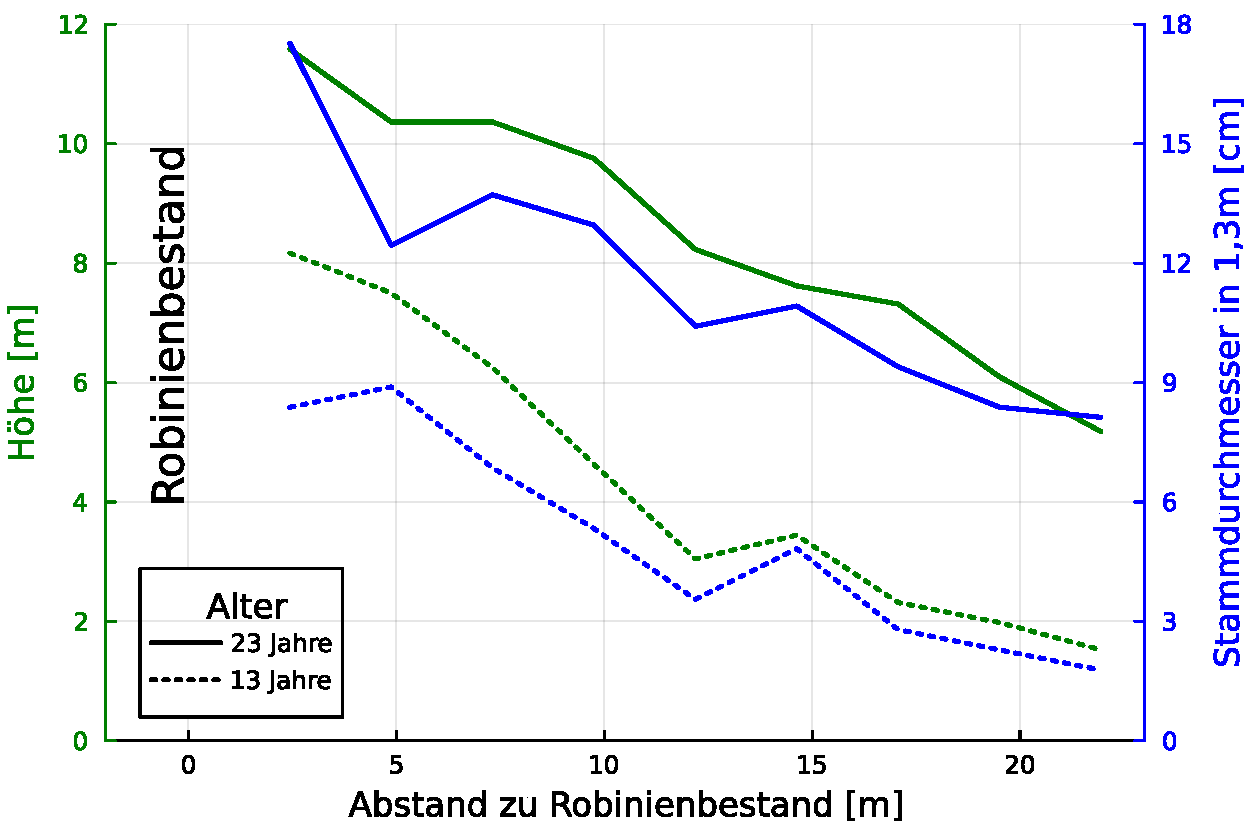
\includegraphics[width=.9\linewidth]{./bild/bestandesrand}
  \caption{Zuwachssteigerung eines Trompetenbaumbestandes an einem
    Robinenbestandesrand nach
    \citet{ferguson1922robinie,chapman1935robinie}}
  \label{fig:bestandesrand}
\end{figure}

Die Veränderungen der Artenzusammensetzung unter Robinien wird eher
durch Veränderungen der Bodennährstoffverfügbarkeit und
Lichtbedingungen verursacht, als durch Allelopathie
\citep{vitkova2017robinie}.  \citet{csiszar2009allelopathy}
untersuchte die allelopathische Wirkung von 15~fremdländischen
Baumarten. Dabei fiel die Robinie, im Gegensatz zu Bastardindigo
(Amorpha fruticosa), Götterbaum (Ailanthus altissima), Zügelbaum
(Celtis occidentalis), Schwarznuss (Juglans nigra), spätblühender
Traubenkirsche (Prunus serotina Ehrh.) und Rot--Esche (Fraxinus
pennsylvanica), nicht durch besondere allelopathische Fähigkeiten auf.

Nach \citet{mueller1991robinie} ist in den
ersten Jahren nach Einbringung der Robinie mit \emph{vorübergehend}
verstärktem Entzug der Hauptnährstoffe Stickstoff, Phosphor und Kali
infolge Nährstoffaufnahme des intensiven Robinienwurzelsytems zu
rechnen. Diese \emph{vorübergehende} Festlegung von Nährstoffen hat
der Robinie den Ruf als \enquote{Nährstoffräuber} eingetragen.
Nach \citet{kou2016robinieBoden} stieg nach einer Ackeraufforstung mit
Robinien der Phosphorgehalt in den obersten 5\,cm, der
Bodenkohlenstoffgehalt in den obersten 60\,cm und der Stickstoffgehalt
bis zur maximalen Untersuchungstiefe von 100\,cm an.
Nach \citet{sitzia2012robinie} wurde die Bodenpflanzendiversität durch
die Robinie nicht reduziert. Unter dem Einfluss der Robinie entwickelt
sich eine Verjüngungshemmende Ruderalflora (siehe
Abb.~\ref{fig:glaswein}).

\begin{figure}[htbp]
  \centering
  \includegraphics[width=.9\linewidth]{./bild/GlasweinRobinie2023a}
  \caption{Robinienversuchsfläche in Glaswein mit üppigem Unterwuchs}
  \label{fig:glaswein}
\end{figure}

Nach \citet[S.~90--92]{erteld1952robinieErtrag} verbessert die Robinie
den Boden erheblich, sodass sich eine artenreiche Bodenflora
entwickeln kann. In dieser Bodenflora haben sich Eiche, Esche, Linde,
Spitz-- und Bergahorn sowie Traubenkirsche eingefunden und zeigen ein
gutes Gedeihen. Im Vergleich dazu fehlen diesen in benachbarten
Kiefernbeständen ohne Robinie. Gerade auf ärmeren Böden wird ein
allmähliches Hineinbringen der Robinie in reine Kiefernbestände
empfohlen.

\citet{kowarik1990robinie} untersuchte die Gehölzsukzession auf
ruderalen Trümmerschuttflächen in Berlin. Die spontanen
Robinienbestände erweisen sich als überraschend gehölzartenreich. Im
Aufnahmematerial sind 77~Gehölzarten enthalten, darunter 38~Baumarten
(z.\,B.\ Vogelbeere, Stiel-- und Traubeneiche, Winterlinde, Feld-- und
Bergulme, Esche, Birke, Eibe), 35~Straucharten und 4~holzige
Kletterpflanzen. Ahorn--Arten sind im Zuge der Sukzession in
Robinienbestände eingedrungen. Birken sterben unter dem Schattendruck
von Robinien ab. Verwilderte Obstgehölze (Apfel, Birne, Nuss, Wein)
kommen ebenfalls neben Robinien vor. Die prägende Strauchart der
Robinienbestände ist der Schwarze Holunder (Sambucus nigra). Er fehlt
in kaum einem älteren Bestand und erreicht Deckungswerte von über
75\,\%. Er ist für die weitere Gehölzsukzession von entscheidender
Bedeutung, da er durch seinen Schatten Gräser und Hochstauden
zuruckdrängt und so das Aufwachsen von schattentoleranten Gehölzen
fördert. Ihr Eindringen in geschlossene mesophile Wälder, in denen sie
noch nicht vorhanden war, ist unwahrscheinlich.

Die Robinie ist im allgemeinen auf Waldstandorten in Deutschland auf
die Dauer einheimischen Holzarten unterlegen. In
Robinienforstgesellschaften ist oft zu beobachten, daß eine starke
Verjüngung von Spitzahorn (Acer platanoides) unter den Robinien
aufkommt. Würde man diese Entwicklung sich selbst überlassen, so wäre
die Robinie bald in ihrem Lichthaushalt so gestört, daß sie meiner
Meinung nach kümmern oder so gar absterben würde
\citep{kohler1963robinie}.

Die beste Strategie zur Eindämmung der Ausbreitung der Robinie besteht
darin, Störungen zu vermeiden, die die Ansiedlung der Robinie
begünstigen, und auf die natürliche Verdrängung der Art durch andere
Bäume zu warten \citep{motta2009robinieBekaempfung}.

Nach \citet{hanzelka2015robinie} sind in Mitteleuropa Robinienbestände
im gesamten Wachstumszeitraum lichter im Vergleich zu einheimischen
Wäldern und sowohl die Strauch-- als auch die Kräutschicht sind daher
dichter. Die Beschattung in Robinienbeständen lag bei 57\,\% im
Vergleich zu 72\,\% in einem einheimischen Eichenwald, die
Strauchbedeckung lag bei 57\,\% im Vergleich zu 11\,\% und die
Krautschicht bei 53\,\% im Vergleich zu 5\,\%.
\citet[S.~47]{bluemke1955robinie} schreibt, dass sich bei 25--30\,m
hohen Robinien mit hohen HD-Wert
(Verhältnis von Baumhöhe zu Durchmesser, hier also dünne hohe Bäume)
durch die Windebewegung und damit
verbundenes abschlagen von Ästen, 1--2\,m breite \enquote{Windschächte}
bzw. Lichschächte zwischen den Baumkronen bilden die dementsprechend
viel licht auf den Waldboden bzw.\ zur Bodenvegetation durchlassen.
Bei Robinen mit niedrigem HD-Wert sind diese Lücken höchsten 0,5\,m
breit bzw.\ können sich die Kronen berühren oder sogar überdecken.
Bei einem von \cite{jessup1791robinie} empfohlenen Pflanzabstand
von 16,5~Fuß (5\,m) werden die Bäume einen niederen HD-Wert haben.

Nach \citet{vitkova2017robinie} ist die Belaubungszeit der Robinie
relativ kurz. Die Blätter erscheinen spät im Frühjahr (Mai) und
beginnen früh zu fallen, normalerweise während der Sommertrockenheit
(August). Die hohe Lichtversorgung ermöglicht es auch lichtbedürftigen
Arten, Frühjahrsgeophyten oder einer dichten Strauchschicht, zu
überleben. Dies dichte Kraut-- und Schrauchvegetation ist jedoch
gleichzeitig ungünstig für die Verjüngung von schattenintoleranten
einheimischen Baumarten sowie auch für die Robinie selbst. Für
Pionierpflanzen ist es typisch, dass sie als Erstbesiedler einen
Standort für nachfolgende Pflanzen vorbereiten, von diesen aber
schließlich selbst verdrängt werden. Bei einer Erhebung einer
Bahnbrache von \citet{kowarik1996robinie} haben sich in fünf Jahren
10~Eichen und fünf Ahorne im geschlossenen Robinienbestand etablieren
können, jedoch nur eine Elche außerhalb.

Die äußerst lichtbedürftige Birke (Betula pendula) dürfte eine der
wenigen Baumarten sein, der die Robinie in Bezug auf Licht tatsächlich
Konkurrenz machen kann, was jedoch Mischungen nicht
ausschließt.
\citet{gaier2009robinieVorverjuengung} berichten von einem
Robinien-Birken-Mischbestand, bei dem im Alter von 60~Jahren
erfolgreich eine Vorverjüngung unter Schirm durchgeführt wurde.  Bei
einem Bestockungsgrad von 0,8 entwickelten sich Winterlinde (Tilia
cordata) und Spitzahorn (Acer platanoides) bei einer von 0,3
Traubeneiche (Quercus petraea) und Hainbuche (Carpinus betulus) etwas
besser.  Die Robinie bildete Wurzelbrut, jedoch konnten keine
negativen Auswirkungen auf den Voranbau festgestellt werden.

Nach \citet[S.~19]{erteld1952robinieErtrag}
gelingt die natürliche Besamung mit Eiche und Edelhölzern
unter dem Schirm der Robinie sehr oft in  hervorragender Weise,
allerdings ist es durch die
Mehrschichtigkeit und die üppige Bodenflora schwierig die Robinie mit
Kiefer zu unterbauen. Mit Fichte und Douglasie ist es mit
entsprechender Pflege eher möglich \citep[S.~94]{erteld1952robinieErtrag}.

Entgegen der weit verbreiteten Meinung, dass die Robinie andere
Baumarten neben sich nicht duldet, hat sich gezeigt, dass sie sich
auch als Mischbaumart eignet. Deshalb wird vielfach empfohlen, in
Reinbestände der Robinie andere Baumarten durch Vor- oder Unterbau
einzubringen \citep{ewald2001klone}.

\citet[p.\,467, 586]{ashton2018silviculture} beschreibt ein
Agroforst-Weidewirtschaftssystem (silvopastoral system) wobei die
Robinie aufgrund ihrer Stickstoffbindungskapazität und ihres lichten
Blätterdaches das Wachstum der darunter liegenden Gräser fördert.

Einmal etablierte Robinien sind aufgrund ihrer Ausschlagfähigkeit
bzw.\ Wurzebrut, insbesondere auf unbewirtschafteten Trockenrasen, aber
auch in lichten Wäldern, schwer wieder loszuwerden. Wobei der Zeitpunkt
der Fällung einen Einfluss auf die Bildung von Stockausschlag und
haben wird. Da sie zu den
Lichtbaumarten mit Pionierkarakter zählt, wird ihre Verjüngung durch
dichten Unterwuchs oder Schattbaumarten stark
eingeschränkt. Schalgflächen kann sie rasch wiederbestocken, ist aber
aufgrund ihrer lichtdurchlässigen Krone kaum in der Lage andere
Baumarten auszudunkeln.

Robinien sind für Pferde giftig \citep{grosche2008robiniePferd}. Sie
wird aber von Hasen und Mäusen geschält bzw.\ deren Wurzeln gefressen,
was Aufforstungen auf Grasland erschwert, und vom Reh verbissen
\citep{barta2023robinieReh}. Nach \citet{berner2018robinie} werden
Robinien von Kühen nicht verbissen. Robinienblätter eignen sich als
Futter für Schafe \citep{ganai2009robnieSchaf}, Ziegen
\citep{papachristou1999robinieZiege} oder Hasen
\citep{singh2010robnieHasennahrung} wobei sie Immunfunktionen bei
Hasen verbessern \citep{yang2017robinieHasen}. Zusätzlich spenden sie
den Tieren Schatten. Insbesondere in trockenen Regionen stehen
Robinien jedoch in Konkurrenz mit anderen Pflanzen um Wasser
\citep{halasz2021robinieAlsTierutter}. So kam es laut
\citet[S.~96]{donaubauer1974kiefernsterben} beispielsweise bei
Schwarzkiefer in Mischung mit Robinie vermutlich aufgrund von
Wasserkonkurrenz zu stärkeren Schäden durch das Ockergelbe
Mehlbecherchen (Cenangium ferruginosum).  Auch Marter in
\citet[S.~93]{erteld1952robinieErtrag} machte die seltene Beobachtung,
dass Kiefern in der Nähe von Robinien rote Nadeln bekamen und
anschließend eingingen.

\section{Verbreitung}

Ihr natürliches Verbreitungsgebiet
befindet sich im mittleren östlichen Nordamerika
(Abb.~\ref{fig:verbreitungNatuerlich}), wobei eine Ausdehnung des
ursprünglichen natürlichen Verbreitungsgebietes durch Ureinwohner möglich
erscheint. Wien ist vom Temperaturgang einzelnen
Herkünften des natürlichen Verbreitungsgebietes ähnlich, die Niederschlagsmenge
ist in Wien jedoch deutlich geringer (Abb.~\ref{fig:wetter}). Auch wenn der
mittlere Monatsniederschlag deutlich höher ist, können dennoch längere Perioden
ohne Niederschlag, insbesondere auf Böden mit geringer Wasserspeicherfähigkeit,
auch in diesen Regionen Trockenstress verursachen.

\begin{figure}[htbp]
  \centering
  \includegraphics[width=.9\linewidth]{./bild/map4}
  \caption{Natürliches Verbreitungsgebiet der Robinie nach \citet{little1971treeAtlas} sowie einzelne Herkünfte}
  \footnotesize{H\dots Harrisburg (Beste Herkunft nach \citet{cobbett1825woodlands}),
    S\dots Long Island (Erstbeschreibung Schifsmastrobinie \citet{raber1936shipmast}),
    X\dots Elkins (Beste Herkunft nach \citet{hopp1941robinie}) sowie Bartow und Thornwood -- Allegheny und Algonquin,
    A\dots Appalachia}
  \label{fig:verbreitungNatuerlich}
\end{figure}

\begin{figure}[htbp]
  \centering
  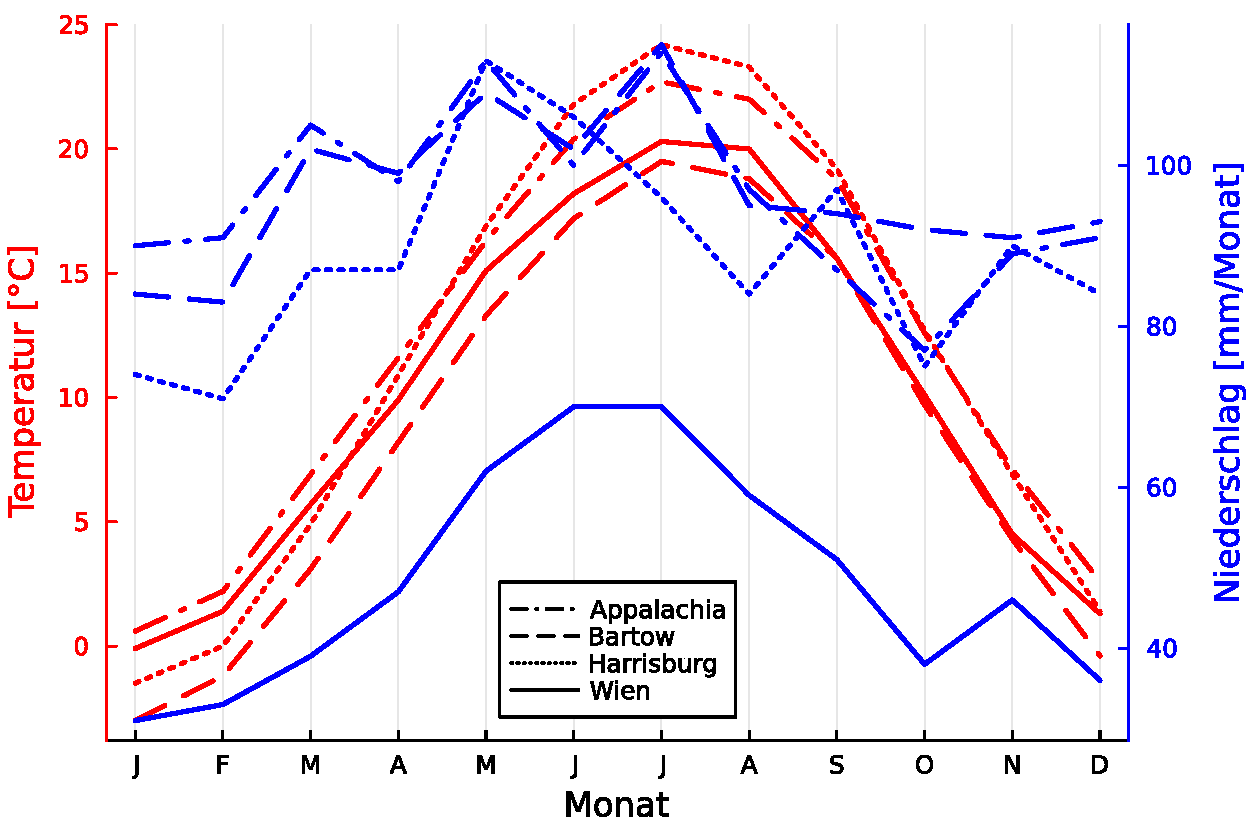
\includegraphics[width=.9\linewidth]{./bild/wetter}
  \caption{Temperatur und Niederschlag dreier Herkünfte sowie von Wien für den
  Zeitraum 1970--2000 abgefraht aus globalen Karten von \citet{worldclim2017}}
  \label{fig:wetter}
\end{figure}

Im laufe der Zeit wurde die Robinie in neuer Regionen gebracht und ist in Europa
und auch global verbreitet (Abb.~\ref{fig:verbreitungGlob},
\ref{fig:verbreitungEuJetzt}). Laut \citet{bouteiller2019robinie} stammen die
Robinien in Europa von vier Populationen aus Nordamerika ab und weisen eine
geringe genetische Vielfalt auf. Die ersten Exemplare wurden im frühen 17.\
Jahrhundert vermutlich aus Virginia eingeführt, während des 17.\ und 18.\
Jahrhunderts kamen weitere aus Pennsylvania und West Virginia hinzu. Diese
scheinen die Mutterpflanzen der meisten, heute in Europa vorkommenden, Robinien
zu sein.

\begin{figure}[htbp]
  \centering
  \includegraphics[width=.9\linewidth]{./bild/verbreitungRobGlob}
  \caption{Verbreitung der 385\,746 Beobachtugnen von Robinie nach \citet{gbifRob}}
  \label{fig:verbreitungGlob}
\end{figure}

\begin{figure}[htbp]
  \centering
  \includegraphics[width=.9\linewidth]{./bild/verbreitungEuropa}
  \caption{Derzeitige Verbreitung der Robinie in der Europäischen Union nach \citet{jrc2016treeAtlas}}
  \label{fig:verbreitungEuJetzt}
\end{figure}

Abbildung~\ref{fig:verbreitungEuPot} zeigt die derzeitige standörtliche Eignung
für Robinien. So gut wie alle Tieflagen in Österreich sind demnach tauglich, was
auch durch registrierte Beobachtungen von Robinie belegt wird
(Abb.~\ref{fig:verbreitungEur}). Für eine waldbauliche Planung ist jedoch
besonders in Zeiten des Klimawandels nicht nur eine derzeitige, sondern auch
eine zukünftige Standortseignung zu berücksichtigen. In
Abbildung~\ref{fig:verbreitungEuPotZukunft} ist die erwartete Standortseignung
der Robinie beim Klimawandelszenarion mit sehr starker Temeraturerhöhung
(RCP~8.5) für das Jahr 2095 dargestellt. Demnach sollten die meisten derzeit in
Österreich für Robinie tauglichen Standorte auch in Zukunft tauglich bleiben.
Selbstverständlich sind solche Schätzungen mit Unsicherheiten verbunden, jedoch
sollte die Gefahr, dass ein Standort seine Tauglichkeit im Lauf der Zeit
verliert, bei Baumarten die relativ kurze Umtriebszeiten erlauben, geringer
sein, als bei solchen mit sehr langen. Die meisten Baumarten sind laut
Forstgesetz erst ab 60~Jahren hiebsreif. Die Robinie ist in der Verordnung für
Raschwüchsige Baumarten aufgenommen, wo die Obergrenze ihrer Hibsunreife mit
10~Jahren festgelegt ist. Umtriebszeiten von 15--30~Jahren sind mit Robinie auf
durchschnittlichen Standorten möglich und lassen sich bei Bedarf durchaus auch
auf 100~Jahre ausdehnen.

\begin{figure}[htbp]
  \centering
  \includegraphics[width=.9\linewidth]{./bild/potentialEuropaAtlas}
  \caption{Derzeitige standörtliche Tauglichkeit für die Robinie in der Europäischen Union nach \citet{jrc2016treeAtlas}}
  \label{fig:verbreitungEuPot}
\end{figure}

\begin{figure}[htbp]
  \centering
  \includegraphics[width=.9\linewidth]{./bild/verbreitungRobEur}
  \caption{Lage der Beobachtungen von Robinie in Europa nach \citet{gbifRob}}
  \label{fig:verbreitungEur}
\end{figure}

\begin{figure}[htbp]
  \centering
  \includegraphics[width=.9\linewidth]{./bild/potentialEuropaZukunft85}
  \caption{Potentielle standörtliche Tauglichkeit der Robinie im Jahr 2095 bei einer Klimaentwicklung nach RCP8.5 nach \citet{mauri2022baumartenZukunft}}
  \label{fig:verbreitungEuPotZukunft}
\end{figure}

Eine gefragte Eigenschaft der Robinie ist ihre relativ hohe Toleranz
gegenüber Trockenheit. Robinien können sich an anhaltende Trockenheit
anpassen, indem sie ihre Spaltöffnungen (Stomata) schließen und sowohl
die Größe einzelner Blätter als auch die gesamte Blattfläche
verringern. Solange jedoch kein Wasserstress besteht, reduzieren sie
ihre Transpiration nicht und gelten daher nicht als wassersparende
Baumart.  Die oberirdische Biomasseproduktion pro Liter Wasser (Water Use
Efficiency, WUE) der Robinie beträgt etwa 2,31~g/L und wenn nur auf das
produzierte oberirdische Holz bezogen 1,63~g/L. Unter Wasserstress
bleibt dieser Wert weitgehend stabil. Damit zählt sie nicht zu
den besonders wassereffizienten Pflanzen, die mit sehr wenig Wasser
viel Biomasse erzeugen können \citep{mantovani2014robinieWasser}.
\citet{lindroth1994wasserverbrauchWeide} gibt für Korbweide (Salix viminalis)
eine WUE von 4,1--5,5~g/L an.
Hingegen \citet{ombodi2022robinieWasserverbrauch} geben für Robinie
eine WUE 1,87~g/L bei ausreichende Wasserversorung aber nur 0,26~g/L bei
hohem Wasserstress an.
Nach \citet{raper1992robinieWasserverbrauch} hat die Robinie einen
WUE von 0,045~g/L,
\citet[S.~126]{lacher2001OekophysiologieDerPflanzen} gibt für
Laubbäume der gemäßigten Zone und für Nadelbäume eine WUE von 3--5~gTS/L an.
Die große Spannweite der von verschiedenen Autoren gemessenen
WUE-Werte für dieselbe Baumart lässt einen Vergleich mit Werten
anderer Baumarten, die ebenfalls von unterschiedlichen Autoren
stammen, unsicher erscheinen.
Da unterschiedliche Klone abweichende Reaktionen auf Trockenstress zeigen
\citep{mapelli2019robinieTrockenstress},
wäre die Angebe welcher Klon untersucht wurde nützlich.

\citet{abri2022robinieTrokenresistenz,abri2023robiieWasser,abri2023robinieDroughtTolerance}
untersuchten für einzelnen Klone die netto Assimilation und die
Transpiration und errechnetet damit die WUE (Tab.~\ref{tab:WUErobinie}).
\citet{abri2025robinieTrockenheit} hat für PL040 im Jahr 2024 eine WUE von
3,64~g/L festgestellt.
Damit wären zumindest bestimmte Sorten sehr effizient hinsichtlich
Zuwachs je verbrauchtem Wasser. Klone mit hoher WUE sollen zumindest
auf wasserlimitierten Standorten höhere Zuwachsleistungen zeigen, was
tendenziell durch die beobachteten Durchmesser-- und Höhenzuwächse bestätigt
wird (Tab.~\ref{tab:WUErobinie}).

\begin{table}[htbp]
  \centering
  \begin{tabular}{l *{7}{S[table-format=1.3]}}
    Klon    &  {NK2} & {Üllöi} & {PL251} & {PL040} & {NK1} \\[.3em]
    WUE Juni 2021 & 6.876 & 6.207 & 6.130 & 7.015 & 4.319 \\
    WUE Juni 2022 &  4.92 & 4.78 & 3.89 & 3.68 & 3.27 \\[.3em]
    iH Mai--Nov 2021 & 2.612 & 1.762 & 2.551 & 2.361 & 1.937 \\
    iH Mai--Aug 2022 & {---} & 1.19 & 1.23 & 1.54 & 1.81 \\[.3em]
    iD Mai--Nov 2021 & 4.09 & 3.89 & 4.09 & 4.24 & 4.08 \\
    iD Mai--Aug 2022 & {---} & 1.873 & 1.997 & 2.376 & 2.135\\[.3em]
    Überlebensrate & 0.84 & 0.52 & 0.64 & 0.72 & 0.70
  \end{tabular}
  \caption{Wassernutzungseffiziennz [g/L] (WUE), Höhenzuwachs [m] (iH) und
    Durchmesserzuwachs [cm] (iD) und Überlebensrate von 2020 bis 2022 verschiedener Robinienklonen die im
    Frühling 2020 gepflanzt wurden
  \citep{abri2022robinieTrokenresistenz,abri2023robiieWasser,abri2023robinieDroughtTolerance}}
  \label{tab:WUErobinie}
\end{table}

Neben dem Wasserverbrauch spielt z.\,B.\ die Interzeption eine Rolle,
also der Anteil des Regenwassers, der in der Baumkrone zurückgehalten
wird und nicht den Boden erreicht.
Nach \citet{gemeinhardt1959robinie} sind die mittleren
Wassergehaltswerte in den durch Robinie meliorierten
Standortsbereichen bis in eine Tiefe von etwa 10\,cm höher als in den
Vergleichsparzellen. In tieferen Bodenschichten wurden keine
Unterschiede festgestellt werden.
Nach \citet{kou2016robinieBoden} wurde ein stillgelegter Acker mit
Spontanvegetation mit einer dort durchgeführten
Robinien-Neuaufforstung verglichen. Unter den Robinien war die
Bodenfeuchtigkeit in den obersten 5\,cm höher, in der Schicht von
5--60\,cm etwa gleich und in 60--100\,cm Tiefe niedriger.

\section{Geschichte}

\subsection{Bis zur Eiszeit}

Im Oligozän~(33,9--23,03~mya; Million Years Ago -- vor
Millionen Jahren) wurden Ablagerungen von zwei Robinienarten in
Europa nachgewiesen. Im Miozän~(23,03--5,333~mya) wurden hingegen mehr
als ein Dutzend Ablagerungen als Robinienart identifiziert. Eine davon
aus dem späten Miozän ähnelt der heutigen Robinie Nordamerikas so
stark, dass ihr Beschreiber geneigt war, beide als identisch
anzusehen. Diese Form war auch während des Pliozäns~(5,333--2,588~mya)
im europäischen Raum verbreitet. Gleichzeitig war an der
Mittelmeerküste Südeuropas eine zweite Robinienart verbreitet. Es gibt
keinen Hinweis, dass diese Robinienarten die erste Eiszeit in Europa
überlebt haben \citep{berry1918robinie}. Während der Eiszeiten
bildeten die Alpen und das Mittelmeer für viele Pflanzenarten in
Europa eine Wanderbarriere. Dadurch wurden vermutlich vor allem
kältetolerante Arten begünstigt, während wärmeliebende und
trockenheitsresistente Arten verdrängt wurden oder ausstarben. Das
verarmte autochthone Artenspektrum könnte in Zeiten starker
Klimaerwärmung den Handlungsspielraum einschränken und ein adäquates
Management erschweren.

\subsection{Erste schriftliche Erwähnungen}

Eine der ersten, wenn nicht sogar die erste, schriftliche Erwähnung der Robinie
(Locust), oder einer Baumart, die ihr ähnlich ist, stammt von Strachey, der dies
zwischen 1610--1612 niederschrieb \citep{strachey1610-1612historie}:
\enquote{The bowes are of some young plant, eyther of the \emph{locust-tree} or
of weech, \dots} (Die Bögen bestehen aus einer jungen Pflanze, entweder aus dem
Locust--Baum oder der weech (witch-hazel -- virginischen Zaubernuss Hamamelis
virginiana), \dots) \enquote{By the dwellings of the salvages are bay-trees,
wild roses, and a kind of low tree, which bears a cod like to the peas, but
nothing so big: we take yt to be \emph{locust}.} (Bei den Behausungen der
Ureinwohner stehen Lorbeerbäume, wilde Rosen und eine Art niedriger Baum, der
eine Schote trägt, ähnlich den Erbsen, aber nicht so groß; für uns sehen sie wie
\enquote{Johannisbrotbäume} aus.)

Sie wurde Anfang des 17.~Jahrhunderts das erste mal nach Europa gebracht und ist
dort mittlerweile weit verbreitet. Jedoch ist derzeit nicht bekannt, wie und
wann genau dies war. Nach derzeitigem Wissensstand wurde sie erstmals 1634 von
John Tradescant dem Älteren in England unter dem Nahmen \emph{Locusta virginiana
arbor} angeführt \citep[S.~339]{gunther1922botanists}. John Tradescant der
Jüngere brachte von einer Reise nach Virginia mehrere Pflanzen mit und könnte
der erste gewesen sein, der Robiniensamen nach Europa gebracht hat. Tradescant
der Ältere war Mitte 1625 in Paris wo ein Austausch stattgefunden haben
könnte \citep{ginter2022robinieGeschichte}.

\citet[S.~171--173]{cornuti1635robinie} beschreibt eine der Robinie
ähnliche Pflanze und gibt ihr den Namen \emph{Acacia Americana
Robini}. In der Beschreibung steht: \enquote{Succedunt semina Lenticulae
similia, quae singula singulis nucleis duris admodum, \& ex omni parte
echinatis clauduntur.} (Die linsenähnlichen Samen sind einzlen in
einzelnen Kapseln eingeschlossen, die sehr hart und auf allen Seiten
stachelig sind.) Die Robinie hat keine Samen die einzeln in einzelnen
stacheligen Kapseln sind.

\citet[S.~28]{deLaBrosse1636robinie} führt eine \emph{Acatia Indica}
an, die angeblich von Vespasien Robin gepflanzt wurde und heute noch
in Paris wächst.

\citet[S.~370]{gunther1922botanists} gibt in einer Liste Samen, die
von Virginia am 18~März 1636 die anscheinend Parkinson von Herrn
Morrice erhalten hat den Eintrag: \enquote{A yellow wood called
\emph{Locust} long flat blackish browne pods, black round flatt seede
kidney like.} (Ein gelbes Holz namens Locust mit langen, flachen,
schwärzlich-braunen Schoten und schwarzen, runden, flachen,
nierenförmigen Samen.), an.

\citet[S.~1550]{parkinson1640theatrumBotanicum} beschreibt die von
\citet{cornuti1635robinie} beschriebene \emph{Acacia Americana Robini}
und gibt ihr den Namen \emph{Pseudoacacia Americana Robini} um diese
von der Robinie, die er \emph{Arbor siliquosa Virginensis spinosa,
Locus nostratibus dicta, Virgin Locus tree} nennt, zu
unterscheiden. Er schreibt: \enquote{A very like tree hereunto hath beene sent and brought us out of \emph{Virginia}, growing to be a very great tree, and of an exceeding height with Masters \emph{Tradescant}, \dots}
(Ein sehr ähnlicher Baum ist uns aus Virginia gesandt und gebracht worden, der zu einem sehr großen Baum mit außergewöhnlicher Höhe heranwächst, bei Meister Tradescant.),
\enquote{We have not seene the tree to bear any flowers with us as yet nor fruite, but the cods that came to us, were small, long, and somewhat flat \dots, containing small grayish flat and round seede.}
(Wir haben den Baum bei uns bisher weder Blüten noch Früchte tragen sehen, aber die Schoten, die zu uns gelangten, waren klein, lang und etwas flach, \dots enthielten kleine, gräuliche, flache und runde Samen.),
\enquote{\dots is called Locus by our Nation resident in Virginia.}
(\dots Wird von unseren in Virginia ansässigen Landsleuten Locus genannt.).

Zur Frage, wann die erste Robinie in Wien angekommen ist, gibt es
unterschiedliche Angaben. Nach \citet[S.~147]{loudon1838arboretum1}
wurde 1696 die erste Robinie im heutigen Palais Pallavicini am
Josefsplatz in Wien
gepflanzt. \citet[S.~15--16]{jacquin1825univGarten} erwähnt neben der
Robinie am Josefsplatz eine weitere, etwa gleich alte Robinie, die von
Kaiser Leopold dem Ersten in der Neuen Favorita in Wieden, der
heutigen Theresianischen Akademie in der Favoritenstraße,
möglicherweise im Jahr 1690, nach Abschluss des Schlosswiederaufbaus,
gepflanzt wurde. \citet{jagr1949robinie} berichtet von einer
300-jährigen Robinie im Gatterhölzl in Meidling, die demnach um 1649
gekeimt wäre. \citet{anonymNatLand1949robinie} erwähnt vermutlich
dieselbe Robinie mit der Altersangabe \enquote{etwa 300-jährige} im
Park der Springervilla in Wien 12., Tivoligasse 73. Die Angabe von 300
Jahren ist demnach nur eine Schätzung, und das daraus abgeleitete
Keimjahr mit Unsicherheiten behaftet. \citet[S.~1395]{hegi1924band43}
nennt die zweite Hälfte des 17.~Jahrhunderts als Ankunftszeitraum der
Robinie in Österreich.
%Die erste Baummieterin in Wien war eine Robinie die 1981 von
%Friedensreich Hundertwasser in der Alserbachstraße~11 gepflanzt wurde.

Über 100~Jahre später schreibt
\citet[S.~339]{Feistmantel1835dieForstwissenschaft} über die Robinie:
\enquote{Obschon sie bereits, allenthalben in Oesterreich verbreitet
  ist, so sieht man sie doch keine eigentlichen Waldbestände bilden.}
\citet{hofmann1851baumloseEbenen} empfiehlt neben vielen anderen
Baumarten auch die Robinie, bei der Anlage von Windschutzhecken zu
verwenden wie dies damals bereits in Schönau in Niederösterreich und
in Altenburg in Ungarn der Fall war.
\citet{hofmann1861waldbaumCulturWarchfelde} beklagt 10~Jahre später,
dass mit wenigen Ausnahmen, Niemand seiner Empfehlung nachgekommen ist
und daher das Marchfeld durch Stürme schwere Verluste erlitten hat.
Auffällig ist, dass 10~Jahre später wesentlich weniger Baumarten
empfohlen werden, nämlich Robinie, Götterbaum, Balsampappel, Eiche,
Schwarz-- und Weißkiefer mit der Bemerkung: \enquote{Im Marchfelde ist
  Alles werthvoll und mit Vortheil benutzbar, was da nur immer
  wächst}.
Laut Angaben der österreichischen Waldinventur
\citep{bfw2025waldinventurWeb} liegt der Vorratsanteil der Robinie in
der Beziksforstinspektion Gänserndorf und Mistelbach bei derzeit bei
ca.\ 12\,\% (Tab.~\ref{tab:waldinventur}).

\begin{table}[htbp]
  \centering
\begin{tabular}{ccc}
Zeitraum   & Robinie  & Ertragswald \\
2000--2002  & 855\,000 $\pm$ 247\,000 & 6\,285\,000 $\pm$ 1\,240\,000 \\
2018--2023  & 950\,000 $\pm$ 328\,000 & 7\,825\,000 $\pm$ 1\,368\,000 
  \end{tabular}
  \caption{Vorrat [Vfm] laut österreichischer Waldinventur \citep{bfw2025waldinventurWeb} in der Beziksforstinspektion Gänserndorf und Mistelbach}
  \label{tab:waldinventur}
\end{table}

\citet[S.~3]{vadas1911robinie} schließt aus alten Bäumen, das
die Robinie erstmals um 1710--1720 in Ungarn gepflanzt wurde, was von
\citet[S.~179]{ernyey1926robinie} angezweifelt wird. Er führt an, dass
János György (Johann Georg Heinrich) Kramer 1735 die Robinie zur
Aufforstung in Ungarn erstmals empfiehlt, wozu es jedoch nicht kommt da
Prinz Eugen von Savoyen, der dies unterstützte, 1736 starb. Nach der
Ungarischen Waldinventur \citep{waldinventur20152019ungarn} der
Periode~2015--2019 stockt die Robinie auf
421\,066\,ha (= 19,2\,\% der Waldfläche) und hat einen stehenden Vorrat von
60\,987\,300\,m³ (= 12,5\,\% des Gesamtvorrats aller Baumarten) und ist
damit bei der Fläche führend und beim Vorrat in etwa gleichauf führend
mit der Zerreiche. \cite{bund1899robinie,gaskil1906robinie} schreiben,
dass jedes Jahr
zwischen fünf und sechs Millionen Robinien gratis zum Pflanzen verteilt wurden,
was zu ihrer weiten Verbreitung beigetragen haben könnte.

\subsection{Selektion und Züchtung}

Auch wenn die genetische Bandbreite in Europa eingeschränkt sein soll, gibt es
dennoch Variationen und so berichtet \citet[S.~259--260]{Michaux1813arbres} von
einer Dornenlosen Robinie (Robinia pseudoacacia spectabilis) welche von
M.~Descemet aus Saint-Denis um 1803--1805 entdeckt wurde und sich besonders gut
für Niederwälder eignen. Zusätzlich soll sie auch noch schneller als die anderen
wachsen. Auch wurde beobachtet, dass Nachkommen aus Samen von dieser donenlosen
Pflanze wieder bedornt waren, aber \citet{Michaux1813arbres} vermutet, dass die
Samen von diesen bedornten Nachkommen dornenlose Nachkommen hervorbringen
werden. \citet[S.~173]{quatrefages1861robinie} beschreibt, dass diese Varietät
vegetativ vermehrt wurde und mittlerweile auf der ganzen Welt zu finden sei.

Robinie lässt sich vegetativ relativ einfach über Wurzelschnittlinge
vermehren. Da die vegetative Vermehrung schon seit langer Zeit
praktiziert wird, kann es vorkommen, dass später gemachte Selektionen,
von verschiedenen Orten, genetisch ident sind
\citep{liesebach2012robinie}. Der Duchmesser von Wurzelschnittlingen
sollte zwischen 1/4 und 1 Zoll (0,6--2,5\,cm) stark sein und Längen
von ca. 3--5~Zoll (8--13\,cm) haben. Die Ausbeute von jungen Bäumen,
vorzüglich jene die in der Baumschule zum Verpflanzen ausgegraben
wurden, ist deutlich besser als jene von alten (bis zu 80\,\% der
Schnittlinge von Jungpflanzen treiben aus).  Bis zu 50\,\% des
Schnittlinge von älteren Bäumen trieben aus, wenn diese Wuzelstärken
zwischen 2--4\,cm hatten.  Der Wuzelschnitt und die Pflanzung sollen
vor dem Austrieb im Frühling erfolgen. Wurzeln müssen vor dem
Austrocknen und vor Frost geschützt werden. Waagrecht gepflanzte
Wurzeln hatten eine höhere Ausbeute gegenüber lotrecht gepflanzten,
was eventuell durch kopfüber Ausrichtungen bei den Lootrechten bedingt
sein kann. Eine lotrechte Wurzelausrichtung führt zu besseren
Jungpflanzen, erfordert aber möglicherweise eine Markierung der
richtigen Ausrichtung. Andererseits verlaufen viele Wurzeln in ihrer
natürlichen Lage waagrecht, insbesondere diejenigen, die im Wald
Wurzelbrut bilden. Arbeitstechnisch ist es effizienter die
Wurzelteile waagrecht in dem Boden zu legen und anschließend zu
bedecken, als diese senkrecht zu pflanzen.
Senkrecht gepflanzte Schnittlinge sollten oben höchstens 1\,cm mit
Erde bedeckt sein. Bei der Wurzelsaat werden 3--5\,cm lange Schnittlinge
waagrecht mit höchstens 4\,cm Erde bedeckt.
Für die jungen beernteten Bäume sind 3--4, 5\,cm lange Wurzelstummel mit Feinwurzeln ausreichend sofern sie in der Baumschule bleiben. Bäume die
im Wald gesetzt werden, sollten ein voll entwickeltes Wurzelsystem,
das weder eingekürzt noch zur Vermehrung über Wurzeln beerntet wurde, besitzen.
Leichte Böden wie sandiger
Lehm eignen sich für die Anzucht, wobei der Boden nicht austrocknen darf.
Bis eine Höhe von 10--15\,cm erreicht ist, sollte ausreichend bewässert werden.
Sprossrückschnitte während des Wachstums sind
schlecht. Stecklinge sowohl aus unverholzten als auch verholzten
Jungtrieben bekommen nur ganz selten Wurzeln
\citep{swingle1937robinie,redei2001robinieVermehrung,redei2005robinieVermehrung}.

Vegetativ vermehrte Pflanzen haben eine geringe genetische Variabilität.
Man versucht dem entgegenzusteuern indem einzelnen Sorten als Klongemisch
angeboten werden. Auch über Samen vermehrte Pflanzen können, wenn diese
von klonaren Beständen kommen, eine geringe genetische Variabilität aufweisen.
Um genetisch vielfältigen Saatgut zu erhalten müssen die beernteten Bestände
heterogen sein \citep{pakull2024robinieKlon}. Ob die daraus gezogenen Bäume
noch die bevorzugt gewünschten Eigenschaften besitzen ist, im Gegensatz
zu den vegetativ vermehrten, jedoch unsicher.

\citet{keresztesi1983robinie} unterteilt ausgewählte Robiniensorten in
die Klassen: Schnittholz (bessere Standorte); Pfähle und Posten
(mittlere Standorte); Imkerei und dekorative Bepflanzung. Manche
Sorten sollen sowohl forstlich als auch zur Honigproduktion geeignet
sein. Für die Honigernte interessant sind frühblüher (var.\ praecox),
spätblüher (var.\ galiana) und dauer-- bzw. öftersblüher
(var. semperflorens Carrière). \citet[S.~80]{crane1986honig} geben ein
Honigpotential von 48--1600\,kg/ha für Robinie an. Zum Vergleich werden
20--42\,kg/ha beim Apfel, 100--200\,kg/ha bei der Salweide,
35--100\,kg/ha beim Raps, 16--200\,kg/ha beim Weißklee oder
25--1000\,kg/ha beim Löwenzahn angegeben.

Robiniensorten wurden von \citet{vilmos1908robiniensorten} beschrieben
und Möglichkeiten der Züchtung erwähnt. Er geht unter anderem auf die
äußeren Form des Baumes sowie die Platzierung und das Wachstums der
Zweige ein.
Die Züchtung der Robinie wurde in Ungarn 1930 von R.~Fleischmann
begonnen \citep{keresztesi1983robinie}. \citet{fleischmann1933robinie}
berichtet, dass die Züchtung hinsichtlich Dürreresistenz eine
reizvolle Aufgabe wäre. Dazu beerntete er lokale Ungarische Robinien,
bekam aber auch Saatgut von amerikanische Provenienzen (Washington,
Staatsforst; Asheville, North Carolina; Jarfield, Ohio; East Lansing,
Mich.). % über Prof.\ Perkins Coville und Prof.\ B.\ A.\ Herbert.
Dabei werden nicht nur Höhen-- und Durchmesserzuwachs, sondern auch
Unterschiede hinsichtlich der Dornenlänge zwischen der verschiedenen
Herkünften beobachtet.
Nach \citet{bloes1992robinie} haben Sorten mit hohen Zuwächsen
tendenziell auch größere Dornen. Durch eine kombinierte Selektion
sollen jedoch sowohl eine hohe Zuwachsleistung als auch eine geringe
Dornenlänge gleichzeitig realisierbar sein.
%Nach \cite{fleischmann1939robinie} ist die
%Robinie reiner Fremdbefruchter und daher variiert die Dornenlänge in
%der Nachkommenschaft.
Auch die Wurzelform (Flach oder Pfahlwurzel) soll ein wichtiges Auslesemoment
für die Robiniezüchtung für trockene Gebiete sein.
Nach \citet{bunger1938robinieWurzeltiefe} können Robinienwurzeln
bis zu 26~Fuß (7{,}9\,m) und nach
\citet[S.~424]{harlow2000dendrology} 20--25~Fuß (6,1--7,2\,m) tief reichen.
Laut \citet{lyr1967wurzel}
können sie bereits in der ersten Vegetationsperiode Tiefen von
1{,}5--2\,m erreichen, was ihnen hilft, Trockenperioden zu überstehen.
Nach \citet[S.~38]{bluemke1955robinie} kann ein einjähriger Sämling eine
Wurzeltiefe von 2,32\,m erreichen.
Mit Bezug auf die
Schiffsmast--Robinie \citep{raber1936shipmast} wird erwähnt, dass auch im
ungarischen Züchtungsplan die Holzqualität sowie Resistenzzüchtungen gegen
Schädlinge aufgenommen sind. \citet{mihalyi1937robinie} schreibt, dass für Ungarn
Saatgut von einem zertifizierten Robinienbestand in Amerika angefordert wurde
und das er ein Paket mit Wurzelschnitlingen der Schiffsmast--Robinie bekommen
hat.
Auch wenn die ersten Publikationen, die ich gefunden habe und die
ausdrücklich das Ziel angeben, geradschaftige Robinien zu züchten, aus den
1930er--Jahren stammen, zeigen beispielsweise einige Abbildungen in
\citet{vadas1911robinie} bereits geradschaftige Robinien, die vermutlich schon um
1850 gepflanzt wurden. Auch \cite{gaskil1906robinie} schreibt das einzelne
Bäume durchaus gerade wachsen.

\citet[S.~67]{wangenheim1781nordamericanischeHolzarten}, der ab 1777
in Nordamerika war, schreibt über die Robinie: \enquote{Dieser Baum
  erwächst ziemlich geschwind, \emph{sehr lang und gerade}, und erhält
  auch eine ansehnliche Dicke. ... Es wird daher lediglich zu Nuzholze
  verwandt.}
\citet[S.~22--23]{wangenheim1781nordamericanischeHolzarten} berichtet
aber auch: \enquote{Dieses bekam die Saamen durch gewisse Personen in
  America übermacht, die nicht die geringste Kenntniß von der Wahl und
  Zeitigung derselben hatten, und dieses Gewerbe blos des Gewinstes
  halber trieben. \dots Teutschland ist bis jezt mehrentheils mit
  solchen ausgearteten, in den englischen Schulen Gärtnermässig
  erzeugten Stämmen verlegt worden.}
\citet[S.~249]{Michaux1813arbres} unterscheidet
zwischen Robinie deren Kern rot (beste Qualität), grün (mittelmäßig)
oder weiß (schlechteste Qualität) ist und vermutete, dass die unterschiedlichen
Färbungen auf die verschiedenen Böden zurückzuführen sind, auf denen die Bäume wuchsen.
Er beschreibt auch, dass auf Long
Island die Wälder im Unabhängigkeitskrieg größtenteils zerstört und
danach Robinien gepflanzt wurden. \citet{cobbett1825woodlands}
beschreibt ebenfalls verschiedene Robinien (Yellow, Sweet, Water),
welche unterschiedliche Holzqualitäten liefern und daher sei auf die
Varietät der Sorte achtzugegeben. Nach ihm kommen die besten
Sorten aus der Nähe von Harrisburg in Pennsylvania, woher er auch
sein Saatgut bezieht. Cobbett war von 1817 bis 1819 auf Long Island
und berichtet von sehr haltbarem Robinienholz und brachte 1819
Robiniensamen nach England und soll davon mehr als eine Million
Robinien verkauft haben. \citet{hicks1883robinie} berichtet von
schwarzen, gelben und weißen Robinien auf Long Island, wobei nur die
gelbe von hohem Wert ist. Die gelbe soll eine grobe Borke bilden,
schwerer durch Samen vermehrbar sein und Höhen von 90~Fuß (27\,m)
erreichen. Diese Robinie soll in Österreich und Ungarn für
Wiederaufforstungen verwendet worden sein. \citet{hopp1941robinie} teilt
die Robinie in die Primärklassen \emph{determinativ} (deutlich ausgeprägter
Stamm, wobei Verzweigungen und Krümmungen entweder fehlen oder
einen festen Charakter aufweisen) und \emph{diffusive} (viele kleine Zweige,
jedoch keinen leicht erkennbaren Stamm) ein, wobei sich zweitere erst
bei Solitären zeigt. Determinativ wird unterteilt nach der Höhe des
Angrifspunktes des Windes (form--point). Damit gibt es die Typen
\emph{pinnate} (gefiedert, determinativ, tiefer form--point --
A-Förmige Krone), \emph{spreading} (ausgebreitet, determinativ, hoher
form--point -- Schirmförmige Krone) und \emph{palmate} (handförmig,
diffusive) ein. Die \emph{besten Herkünfte} stammen aus der pinnate Klasse,
welche \emph{im natürlichen Verbreitungsgebiet nur in Elkins, West Virginia
in Hochlagen} gefunden wurden. Spreading bildet fast nur krumme
Schäfte. Im Dichtstand ist die Stammform von Palmate auch recht gut
wohingegen Pinate den Dichtstand weniger gut verträgt.

Nach \citet{detwiler1937robinie} macht \emph{Charles F.\ Swingle} 1934
den Vorschlag die gelbe Robinie wegen ihres langen, geraden Stammes,
als \emph{Schiffsmast--Robinie} (\emph{Shipmast Locust}) zu
bezeichnen. Dieser Name wurde von \citet{raber1936shipmast} erstmals
publiziert, ohne zu erwähnen, dass die Idee dieses Namens nicht von ihm
stammt. Er vergibt der Varietät den Namen \emph{Robinia pseudoacacia
var.\ rectissima}. Diese soll auch im Freistand gerade wachsen und
Höhen bis 100~Fuß (30\,m) erreichen. Diese soll man in New Jersey, New
York, Long Island und Massachusetts finden. Ihr Holz soll dauerhafter,
die Krone schmäler, die Rinde gröber, der Zuwachs größer und die
Resistenz gegen Insekten besser sein. Sie bildet wenig Blüten, der
Pollen keimt wenig und der Baum hat wenig bis keine Samen, sodass sie
überwiegend vegetativ vermehrt wird.
%Dies soll darauf hindeutet, dass die Schiffsmast--Robinie möglicherweise ein Hybrid oder ein steriler Klon ist.
Nach \citet{hopp1941robinieUnterschied} hat die
Schiffsmast--Robinie kleinere Dornen und breitere Blätter. Auf
geringwüchsigen Standorten ist der Zuwachs der gewöhnlichen Robinie
besser als der der Schiffsmast--Robinie, bei welcher der Wipfel
abstirbt und sich der Höhenzuwachs einstellt.
Nach \citet{hopp1947robinie} liegt die gewöhnliche Robinie bis zum Alter~50
beim Zuwachs vor der
Schiffsmast--Robinie. Danach nimmt der Zuwachs der gewöhnlichen
Robinie ab, während die Schiffsmast--Robinie hohe Zuwachsraten
beibehält.

\citet{hirt1938robinie} und \citet{toole1938robinie} verglichen die
Resistenz von normalen mit der Schiffsmast--Robinie gegenüber
holzzerstörenden Pilzen, wobei die Schiffsmast--Robinie bei zwei von
vier untersuchten Pilzen resistenter war.
Nach \citet{duenisch2009robineHolzJungAlt} haben die ersten
10--20~Jahrringe, die der Markröhre anliegen, eine deutlich geringere
Resistenz gegenüber Pilzen als das übrige Kernholz. Das in der Jugend
des Baumes angelegte Kernholz verlor innerhalb von 16~Wochen
durchschnittlich 17,0,\% an Holzmasse, während das im höheren Alter
gebildete Kernholz nur um 1,7,\% abnahm. Dabei streut die Abbaurate im
marknahen Holz stark und dürfte von den Standortsverhältnissen sowie
dem Genotyp des Baumes beeinflusst werden \citep{brischke2024robineDauerhaftigkeit}.
\citet{szczepkowski2025robinePilze} stellten ebenfalls fest, dass die
Widerstandsfähigkeit von Robinienholz mit zunehmendem Alter deutlich
zunimmt.
Auch die Holzfestigkeit ist im innersten Kern der ersten 7--11~Jahre
reduziert, während sich die Holzdichte hingegen kaum unterscheidet
\citep{adamopoulos2007jungesUndAltesRobinienholz,bijak2021robinienholz}.

\citet{hall1937robinie} beschreibt, dass ein großer Anteil der in den
Vereinigten Staaten gepflanzten Bäume aus in Europa beerntetem Saatgut
produziert wurde. Bei Saatgut aus Amerika wurden auch kleinen,
minderwertigen und oft vom Robinienbock befallene Bäume beerntet. 1935
wurde die Resistenz der Schiffsmast--Robinie im Vergleich zur
gewöhnlichen untersucht mit dem Ergebnis, dass die
Schiffsmast--Robinie weniger anfällig gegenüber dem Robinienbockkäfer
ist und die Anfälligkeit mit zunehmender Bonität abnimmt.
\citet{wollerman1968robinieBorer} beobachtete, dass im ersten Jahr
resistent erscheinende Klone im nächsten Jahr befallen wurden.
Von den zehn verglichenen Klonen, darunter offenbar auch Appalachia,
Allegheny und Algonquin, wies Klon~4193 (dürfte BN-4193 = HC-4148 sein,
welcher wie Allegheny aus Barton kommt
\citep{santamour1960robinie,steinergroup1987robinie}) auf der stark befallenen
Fläche mit durchschnittlich 10~Robinienbockkäfern pro Baum den
geringsten Befall auf. Der nächstbeste Klon (Nr. 8450) hatte 22~Käfer
pro Baum, während Appalachia mit 38~Käfern am stärksten betroffen war.
Für belastbare Aussagen sind langfristige und standortsübergreifende
Beobachtungen nötig.

Einigkeit herrscht darüber das die von Long Island
bechriebenen Schiffsmastrobinien gepflanzt und vorher offensichtlich
irgendwo zur Vermehrung selektioniert wurden. Manche vermuten, dass sie
aus Virginia stammt (\citet{hicks1883robinie} vor über 100~Jahren,
\citet{raber1936shipmast} um 1700, \citet{detwiler1937robinie} 1683),
andere schreiben, dass es unklar ist, woher sie stammt
(\citet{raber1938robinie}). \citet{detwiler1937robinie} beschreibt,
dass nach wie vor noch bessere Robinien selektiert werden und dass
1934 eine staatliche Baumschule in North Carolina die Vermehrung von
Schiffsmast--Robinien betreibt.
%\cite{raber1936shipmast} schreibt ebenfalls das John Sands
%diese Robinien nach Lang Island gebracht hat.  \cite{raber1938robinie}
%beschreibt er dei Möglichkeit dass Kapitän John Smith um 1700 Robinien
%auf Sand Point von wo sie weiter verbreitet wurde. Er kommt zu dem
%Schluss, dass es unklar ist woher diese Robinie stammt, sowie wann und
%von wem sie nach Long Island gebracht wurde und dass sie mittlerweile
%in weiten Teilen der USA zur Verringerung der Erosion verwendet
%wird.
\citet{cope1938robinie} beschreibt, dass man die Schiffsmast-Robinie im
gesamten Hudson-Tal findet, ihre Wipfel jedoch in einem kalten Winter
abgefroren sind, mit Ausnahme offenbar frostharter Varianten in
Saratoga und Washington, die nach seiner Ansicht für die Vermehrung
besser geeignet sind.
\citet{minckler1948robinie} berichtet von einer Aufforstung in Illinois
im Jahr 1935 bei der Samen des besten lokalen natürlichen Bestandes
und Wurzelschnittlinge der Schiffsmast-Robinie aus Long Island
verwendet wurden. Ein Vergleich der beiden im Jahr 1948 zeigte keine
wesentlichen Unterschiede in Form oder Wachstum.

Nach \citet{santamour1970robinie,steinergroup1987robinie} wurden von 1938 bis 1943 über 100
Robinienklone gesammelt, welche hohes Wachstum und eine gute Stammform hatten
und wenig vom Robinienbock befallen wurden. Die meisten der untersuchten
Bestände lagen außerhalb des natürlichen Verbreitungsgebiets der Robinie und
hatten sich aus alten Pflanzungen entwickelt \citep{hopp1941robinie}. Die
gesammelten Klone wurden von 1943 bis 1950 in Beltsville, Maryland getestet. Von
diesen wurden fünf ausgewählt, worunter auch die Schiffsmast--Robinie aus Long
Island war, welche aber sowohl bei Zuwachs, Resistenz, Astreinigung als auch
Geradschaftigkeit schlechter als die anderen war \citep{santamour1960robinie}.
1950 wurden 15 weitere Klone aus einheimischen Beständen hinzugefügt.
Zwischen 1948 und 1965 wurden 46 Testpflanzungen der ausgewählten
Klone angelegt. Viele der Pflanzungen enthielten weniger als zehn Klone,
und nur in Cape May waren alle 20 Klone vertreten Fünfzehn davon wurden
1985 von Ruffner lokalisiert und gemessen \citep{bongarten1992robinie}.
Dabei wurden die 3~Klone Appalachia, Allegheny und Algonquin ausgewählt,
welche aus der Gruppe der 5 bereits 1950 ausgewählten Klone stammen.

\begin{description}
  \item[Appalachia:] (HC-4138; BN-4191; NA-4913; 9030613) wurde zwischen
Blackwood und Appalachia in Virginia (ca.~36,91N; 82,70W) entdeckt und 1956
benannt, hat ausgezeichnetes Wachstum und Form, ein Klon, Stamm gerade,
zylindrisch, Äste dünn, gut verzweigt, gute Astreinigung, stärker verbissen,
85\,\% Schnittholz, \citep{steinergroup1987robinie,zsombor1980robinie,kapusi1995robinie}.
  \item[Allegheny:]  (HC-4146; BN-4192; NA-4914; 9030614) kommt aus der Nähe von
Bartow in West Virginia (ca.~38,54N; 79,78W), wurde 1987 benannt, hat
ausgezeichnete Vitalität, gerade, unverzweigte Stämme und einen
überdurchschnittlichen BHD sowohl in der Jugend als auch im Alter \citep{steinergroup1987robinie}.
  \item[Algonquin:] (HC-4149; BN-4194; NA-4916; 9030615) kommt aus der Nähe von
Thornwood in West Virginia (ca.~38.56N; 79.74W) und wurde ebenfalls 1987 benannt
hat die beste Wuchsleistung und überdurchschnittliche Resistenz gegen den
Robinienbock \citep{steinergroup1987robinie}.
\end{description}

Die Fundorte von Allegheny und Algonquin dürften ca.\ 2\,km
voneinander entfernt liegen und diese liegen ca.\ 50\,km entfernt von Elkins wo
nach \citet{hopp1941robinie} die beste Herkunft im natürlichen Verbreitungsgebiet
zu finden ist.  Damit eine gewisse genetische Heterogenität besteht, sollen alle
drei Klone gemeinsam gepflanzt werden, wobei für Algonquin ein Anteil von
50--80\,\%, aufgrund ihrere hohen Wuchsleistung, empfohlen wird. Diese
Klonmischung wurde Steiner Group, nach dem Züchter Wilmer W.Steiner, genannt.
Die von \citet{liesebach2012robinie}
untersuchten Proben der Klone Allegheny und Algonquin waren identisch und
stimmten auch mit einer früheren Lieferung von Appalachia überein, wohingegen
sich eine neue Lieferung von Appalachia von den anderen genetisch unterschied.
Diese Übereinstimmung kann jedoch auch daher kommen, da die
Mikrosatellitenmarker nur sehr kleine Ausschnitte des Kerngenoms erfassen. In
\citet{liesebach2021robinie} wird zwischen Appalachia--4191 und Appalachia--4138
unterschieden. Nach dem \citet{steinergroup1987robinie} gibt es eine
ursprüngliche SCS--Soil Conservation Service Hillculture (HC) und eine spätere
Beltsville (BN) Nummerierung und für Appalachia gibt es demnach BN-4191 und
HC-4138 welche den identen Klon bezeichnen. Zusätzlich gibt es noch eine NRCS
(Natural Resources Conservation Service) Nummer die für Appalachia 9030613 ist,
eine NA Nummer welche für National Arboretum stehen dürfte mit NA-4913 und auch
eine vom Morris Arboretum mit 50-308.

Geradewüchsige Robinie sind schon lange bekannt und es gab einen
Austausch von ausgewähltem Vermehrungsgut (Samen und
Wurzelschnittlinge). Nach \citep{keresztesi1983robinie} gingen die
Experimente von R.~Fleischmann im Zweiten Weltkrieg verloren, dennoch
zeigt er auf S.~224 eine Abbildung von 44~jährigen rectissima Robinien
im Gödöllö Arboretum, welche wohl aus den Wurzelschnitlingen, die
\citet{mihalyi1937robinie} aus Amerika erhalten hat, stammen.  Die
Züchtung wurde 1951 in Budapest von F.~Tuskò und B.~Keresztesi wieder
begonnen und 1955 von F.~Kopecky verstärkt. Ziel war es einerseits,
schnellwachsende, geradwüchsige und frostresistente Bäume auszuwählen,
andererseits solche mit verlängerter Blütezeit und erhöhtem
Nektarertrag \citep{redei2007robinieSelektion,csiha2016robinie}.
Eine Klonbank wurde eingerichtet um Klonuntersuchungen
und Kreuzungsexperimente durchzuführen. Zusätzlich wurde in allen
Robinenwäldern Ungarns nach geradewüchsigen Robinien gesucht und
Ableger in Gödöllö getestet und anschließend die besten vegetativ
vermehrt. 1964 wurden 134 dieser geradewüchsigen Varietäten gepflanzt
und verglichen.  Derzeit gibt es in Gödöllö auf 50~Hektar, 210~Klone
und Sorten \citep{redei2005robinieVermehrung,csiha2016robinie}.

\citet{keresztesi1974robinie} zeigt eine Auswertung von 7~Sorten
hinsichtlich Zuwachsleistung wo insbesondere Nyirségi, Röjtökmuzsaji
und Üllöi hervorstechen. Zusätzlich werden eine Grafik 32~Robiniensorten
hinsichtlich 4 Qualitätsstufen (sehr gut, gutes Schnittholz,
Rebpfähle, Brennholz) beschrieben. Hier überzeugen
Jászkiséri (92\,\%Schnittholz)
, Pénzesdombi (90\,\%)
, Appalachi (86\,\%)
, Zalai (83,5\,\%)
, Nyirségi (82,5\,\%)
, HC--4146 = Allegheny (82\,\%). Es werden auch
Üllöi (57\,\%)
, Rectissima (50\,\%)
, HC--4149 = Algonquin (46,5\,\%)
oder HC--4148 (42,5\,\%)
angeführt.
Eine Zusammenfassung davon ist auch in \citet{keresztesi1983robinie} zu finden.
Dies zeigt dass die Selektionen aus Amerika oder Rumänien
fast zeitgleich in Ungarn angekommen und geprüft wurden.
\citet{bluemke1955robinie} berichtet das der Klon HG--4138 aus Blackwood (was
vermutlich HC--4138 sein sollte und damit Appalacia wäre) in Holland
für den Handel freigegeben wurde.

\begin{description}
  \item[Zalai:] 1973 in Ungarn registriert \citep{keresztesi1983robinie}
  \item[Nyirségi:] 1973 in Ungarn registriert, 6--Klone, kräftige Krone, Dichtstand da sie sonst zur Verzweigung neigt, bei Weitverband Astung, Dornenlänge 13\,mm, geringe Samenproduktion \citep{keresztesi1983robinie,kapusi1995robinie,abri2024dis}
  \item[Rozsaszin~AC:] 1973 in Ungarn registriert, 6--Klone, Rosa Blüte, Honig \citep{keresztesi1983robinie,kapusi1995robinie}
  \item[Jászkiséri:] 1979 in Ungarn registriert, 1--Klon, starkwüchsig, große Krone, dicke Äste, Dornenlänge 19\,mm, neigt zur Verzweigung => Dichtstand, geringer Ligningehalt \citep{keresztesi1983robinie,zsombor1980robinie,kapusi1995robinie,abri2024dis}
  \item[Kiskunsági:] 1979 in Ungarn registriert, gerader zylindrischer Stamm, dünne Äste, große Dornen, 41\,\% Schnittholz \citep{keresztesi1983robinie,zsombor1980robinie}
  \item[Pénzesdombi:] 1979 in Ungarn registriert, aus Rumänien, sehr schnellwüchsig, 66\,\% Schnittholz, wenige, kleine Dornen, \citet{zsombor1980robinie}
  \item[Csázátötélési:] 1979 in Ungarn registriert, gerader Stamm, dünnastig, große, Dornen, früher Austrieb, 37\,\% Schnittholz \citep{zsombor1980robinie}
  \item[Appalachia:] 1979 in Ungarn registriert, aus Amerika
  \item[Üllöi:] 1982 in Ungarn registriert, aus Üllő Forstabteilung 10D von J.~Fila, 3--Klone, gerader Stamm, 44\,\% mehr Holzmasse der besten Qualität, Dornenlänge 10\,mm, geringe Samenproduktion, \citep{bach1983robinie,kapusi1995robinie,abri2024dis,redei2020ulloi}
  \item[Debreceni-2:] 1979 in Ungarn Kandidat \citep{keresztesi1983robinie}
\end{description}

Für die Schnittholzproduktion sollen sich Nyirségi, Kiskunsági, Jászekiséri,
Pénzesdombi, \emph{Röjtökmuzsaji}, \emph{Góri} und Appalachia gut eignen, wobei
Kiskunság auch viel Honig produziert. Neben Wuchsform und Wuchsleistung wurde
auch nach Resistenzen (Spätfrost, Virus, Insekten) selektiert.

In den 1980er Jahren wählte Imre Kapusi ca.\ 50\,000 einjährige
besonders große Sämlinge aus, von welchen im Alter 8--12~Jahre die
besten 125 selektiert wurden. Aus dem Saatgut dieser 125 wurden nach
weiteren 17~Jahren 70~Plusbäume ausgewählt (OBE01--OBE70?) welche die
Basis der Sorte \emph{Turbo Obelisk} bilden, von denen OBE26, OBE34,
OBE53, OBE54 und OBE69 registriert sind.
%Von denen sind OBE26, OBE34,
%OBE53 am geradesten und haben große Zuwächse (pers.\ Auskunft
%15.\ Feb.\ 2024 Viktor Jósa).
Pflanzen aus dem Saatgut dieser 70~Klone bilden eine Samenplantage aus
der \emph{Turbo} Sämlinge gewonnen werden \citep{nemeth2022robinie}.
Vergleiche zwischen einigen der 125 anfänglich selektionierten (A) und
deren Folgegeneration (B) wurden von \citet{barna2009robinieTurbo}
durchgeführt, wobei (A) die ersten drei Plätze hinsichtlich
Höhenwachstum hatten. Eine Selektion von (B) hatte den stärksten
Durchmesserzuwachs gefolgt von zwei Selektionen aus (A).

\begin{description}
  \item[Turbo:] Sämling, Schneelwüchsig \citep{nemeth2022robinie}
  \item[Turbo Obelisk:] 3--Klone (OBE26, 34, 53), 5--Klone (OBE26, 34, 53, 54, 69), Schneelwüchsig, geradschaftig \citep{nemeth2022robinie}
\end{description}

Nach \citet{redei2008robinieImprovement} kann nur auf Standorten mit
ausreichender Feuchtigkeit und gut durchlüfteten, möglichst leichten,
nährstoff-- und humusreichen Böden gute Qualität erzeugt werden. Um
das Standortsspektrum zu erweitern wurde in
den 1990er Jahren unter der Leitung von Károly Rédei
hinsichtlich Dürreresistenz selektiert mit den Sorten:
\begin{description}
  \item[Vacsi:] PV~201E~2/1, aus Pusztavacs, gerader Stamm, mittlere Wuchskraft,feinastig, kleine Dornen
  \item[Szálas:] Dürreresistet
  \item[Oszlopos:] PV~233A/1, aus Pusztavacs, gerader Stamm, mittlere Wuchskraft, Dornenlänge 1--3\,mm
  \item[Homoki:] MB~17D~3/4, aus Mikebuda, leicht gebogener Stamm, starkwüchsig, Dornenlänge 5--8\,mm
  \item[Bácska:] KH~56A~2/5, aus Kéleshalom, neigt zu Zwiesel, starkwüchsig, Dornenlänge 6--12\,mm
\end{description}
wovon besonders Vacsi, Homoki, Bácska und PV201E2/4 hinsichtlich Qualität und Wuchsleistung vielversprechend
sind \citep{redei2018robinieImprovement,keserue2021robinie,abri2023robinieUngarn,abri2024dis}.

In den späten 2010er Jahren wurde weiter in Richtung Dürreresistenz
gekoppelt mit schnellem Jungedwachstum und hoher Stammqualität
selektioniert mit den Sorten \citep{abri2023robinieUngarn,abri2024dis}:
\begin{description}
  \item[PL251 -- Püspökladányi:] gerader zylindrischer Stamm, gutwüchsig, kurze Dornen
  \item[PL040 -- Farkasszigeti:] gerader zylindrischer Stamm, feinastig, mittlere Wuchskraft, große Dornen
  \item[NK1 -- Laposi:] annähernd gerader Stamm, mittles Höhen-- und starkes Dickenwachstum, kleine Dornen
  \item[NK2 -- Napkori:] gerader zylindrischer Stamm, starkwüchsig,
feinastig, kleine Dornen
\end{description}
Diese waren hinsichtlich Durchmesser-- und Höhenzuwachs Üllöi in der
Jugend überlegen.

\citet{schroeck1953robine} führt die geringe Wertschätzung der Robinie
auf ihre Krummwüchsigkeit zurück, welche sich aber durch Züchtung
beheben lässt. Im Lehr-- und Versuchsrevier Sauen, Schlepke sowie im
Bauernwald Hasenholz fanden sich Klone mit völlig geraden
Schäften. \citet{erteld1952robinieErtrag} erwähnt neben dem
Revier Sauen auch die Revierförsterei Spitzberg mit geradschaftigen Robinien.
In Sauen soll Geheimrat Bier bzw.\ sein Sohn Prof.\ August Bier 
von besonders guten Mutterbäumen Einzelstammabsaaten angelegt haben.
Neben Klonen aus dem Revier Buckow werden in
\citet{naujoks2005robinie} auch Klone aus dem von
\citet{schroeck1953robine} schon erwähnten Revier Sauen aufgezählt.
\citet{naujoks2005robinie,hofmann2020robinie,lange2021robinie,lange2022robinie}
berichten von einem Anbauversuch, bei dem auf 4~Versuchsflächen
12~vorausgelesene Robinienklone, drei Bestandesabsaaten und zwei
Plantagenabsaaten im Winterhalbjahr 2013/2014 gepflanzt wurden. Dabei
war von manchen bekannt, dass sie aus Ungarn stammen, nicht jedoch
deren Sorte, welche durch gentechnische Untersuchungen zum Teil wieder
zugeordnet werden konnten. Die Sorte Kiskunsági wurde nicht vegetativ
sondern über Samen vermehrt verwendet. In den 1990er Jahren wurden in
Brandenburg 33 wüchsige und geradschaftige Robinien--Plusbäume, die
kaum oder keine Starkäste hatten, ausgelesen, von denen sechs als
Gewebekulturklone etabliert und in den Versuch aufgenommen wurden
(Robert, Roger, Romy, Rowena, Roy). Auch die Sorten Bendida und Tangra
der Firma Lignum in Bulgarien Bulgarien und Cuci aus Rumänien wurden
verwendet. Dabei wurden Unterschiede hinsichtlich Vitalität im Alter~5
erhoben wobei Appalachia, Nyirségi und Fraport3 (=Zalai?) auf zwei
Probeflächen die höchsten Anteile voll vitaler Bäume
hatten. Hinsichtlich Steilästen waren Bendida (45,4\,\%) Fraport3
(46,3\,\%) Romy (50,0\,\%) Cuci (51,9\,\%), hinsichtlich
Wipfelschäftigkeit waren Fraport3, Appalacia, Nyirségi, Bendida, Romy
und hinsichtlich geradschaftigkeit Fraport3, Jászkiséri, Appalacia,
Bendida, Nyirségi die besten.  Hinsichtlich Höhenzuwachs in 6 Jahren
waren Fraport3 (7,54\,m), Roger (6,93\,m), Rowena (6,84\,m) und
Appalacia (6,76\,m) die Zuwachsstärksten. Im Trockenjahr 2018 hatten
Appalacia (0,86\,m), Roy (0,73\,m), Romy (0,72\,m), Rowena (0,70\,m)
und Fraport3 (0,68\,m) die größten Höhenzuwächse.  Die größten
Biomassezuwächse in 6~Jahren hatten Fraport3 (6,9 t/ha), Roger (6,1
t/ha) und Romy (6,1 t/ha).

In Polen wurden in Jahr~2014 28~geradschaftige Klone aus 7~Beständen
geworben. Die Bestände sind: Krosno--90b, Krosno--232i, Cybinka--98y,
Wołów--194f, Pińczów--426f, Strzelce--150Am, Mieszkowice--210j und
Wyszanów \citep{wojda2015robiniePolen}.

Große Gebiete in Korea wurden mit Robinie aufgeforstet um die
Bodenerosion einzudämmen. 70\,\% der Honigproduktion kommt von der
Robinie. Als geradschaftige Selektionen werden Hapcheon und Daegu
angegeben \citep{lee2007robinieKorea}.

Vergleichsanbauten mit fremdländischen Baumarten wurden in Österreich
von \citet{cieslar1901fremdlaendischeHolzarten} publiziert. Robinien
wurde dabei nicht untersucht. Auch in Deutschland wurde die Robinie
beim Vergleich fremdländischer Baumarten
nicht untersucht \citep{schwappach1901fremdlaendischeHolzarten}.
\enquote{Auf Grund der guten Erfahrungen, die bisher mit in heimischen
Wäldern angebauten Weymouthskiefern, Robinien, der amerikanischen
Schwarznuß und Roteiche sowie Douglasien gemacht worden sind, spricht
sich Cieslar für die Durchführung von Anbauversuchen mit Exoten aus
und kündigt von der Versuchsanstalt geplante Exotenkulturversuche
an. \dots Von der Exoten-Inventur ausgeschlossen waren die Robinie und
die verschiedenen Pappelarten, da diese wegen ihrer weiten Verbreitung
im östlichen Österreich schon als "heimisch"\ betrachtet werden
konnten} \citep{rannert1979fremdlaendischeBaumarten}. Solange es
darum geht, zu prüfen, ob eine Baumart in einer neuen Region überhaupt
wächst, mag diese Beschränkung gerechtfertigt sein.
Wenn jedoch die Baumart mit der besten Leistung gesucht wird,
müssen alle vielversprechenden Baumarten,
sowohl heimische als auch fremdländische, gepflanzt und miteinander verglichen werden,
wie es bereits von \citet[S.~300]{reaumur1721ertragstafel} gefordert wurde:
\enquote{Il ne faudroit commencer qu’à défricher de très-petits cantons , \& à les planter de différentes sortes d'Arbres, pour voir ceux qui y réussiraient mieux.} (Man sollte zunächst nur sehr kleine Flächen roden und sie mit verschiedenen Baumarten bepflanzen, um herauszufinden, welche dort am besten gedeihen.)
\enquote{Enfin il faudroit tâcher de reconnoître les terrains les plus  propres à chaque espéce d’Arbres , \& ne leur donner que Les espéces d’Arbres qui leur sont propres.} (Schließlich sollte man versuchen, die Böden zu erkennen, die am besten für jede Baumart geeignet sind, und ihnen nur die Baumarten geben, die zu ihnen passen.)
\enquote{Notre attention ne devroit-elle pas aller jusques à chercher si les pays étrangers n'ont point des Arbres qui nous seroient utiles, qui croîtroient aisément dans le Royaume?} (Sollte unsere Aufmerksamkeit sich nicht sogar darauf richten, zu prüfen, ob es nicht Bäume aus fremden Ländern gibt, die für uns nützlich wären und die leicht im Königreich gedeihen würden?)
Auch \citet[S.~253]{carlowitz1713sylvicultura} zog in Erwägung fremdländische
Baumarten zu verwenden wenn diese gute Eigenschaften hatten: \enquote{\dots und daß das Europäische, jenen an der Güte nicht gleichet / und also ein mehrerer Nutzen / vielleicht durch Fortpflantzung derer frembden wilden Bäume / als durch zarte ausländische Gewächse / entstehen könte / auch das wilde Holtz / weil es dauerhaffter  und stärckerer Natur ist / desto eher als jene / zumahl durch den Saamen fortbracht werden möchte.  \dots  das uns nutzbare Indianische oder andere frembde Holtz / auch in Europa aufbringen zu lassen.}

In Österreich wurden in den 1980er Jahren von Ferdinand Müller die
Sorten \emph{Tulln} hinsichtlich Biomasseerzeugung im Kurzumtrieb
selektioniert. Wuchsform war kein
Selektionskriterium. \citet{mueller1999robinie} hatte das Ziel ein
Klongemisch, eine Mehrklonsorte zu schaffen, die aus etwa 30~Klonen
zusammengesetzt ist und bezieht sich dabei auf
\citet{huehn1986klonanazahl} der je nach erwarteter Ansteckungsgefahr
20--40 Komponenten empfiehlt.
\enquote{Derzeit wird angestrebt, die
  bisher zehn wüchsigsten Klone in einer größeren Zahl für breiter
  gestreute Anbauversuche zu vermehren und weitere Klone zur Erhöhung
  der Klonzahl auszuwählen. Erst wenn 30 auf mehreren Standorten
  geprüfte Klone zur Verfügung stehen, wird die Verwendung des
  Pflanzenmaterials empfohlen werden können. Selbst dann wird aber ein
  steter Wandel der Klonzusammensetzung durch Ausscheiden weniger
  geeigneter Klone zugunsten von leistungsfähigeren Auslesen eine
  Variation der Genotypenzusammensetzung künftiger
  Kurzumtriebsplantagen gewährleisten.} \citep{mueller1999robinie}.
Vergleichsanbauten wurden 1982 in Karlwald bei Halbturn und Rüsterwald
bei Neusiedel, 1985 in St.~Margarethen und 1988 in Riedenthal bei
Mistelbach angelegt. Kurzumtriebsflächen wurden 1984 in Wasserburg bei
St.~Pölten und 1985 in Bruckneudorf, Biomasseversuche 1987 in
Neckenmarkt und 1988 in Nickelsdorf angelegt.  Eine Auswertung einer
1985 im Versuchsgarten Tulln angelegten Biomasse--Versuchsfläche ergab
bei einer 4~jährigen Umtriebszeit eine Trockenmasseproduktion im
Mittel über alle österreichischen Selektionen 7,44~t/ha/Jahr, bei den
zehn wüchsigsten 10,07~t/ha/Jahr bei Appalachia 5,93~t/ha/Jahr und bei
Nyirségi 4,07~t/ha/Jahr \citep{mueller1991robinie}.
Nach \citet{redei2005robinieEnergieholz} ist der Ertrag im ersten
Umtrieb geringer.
Publiziert wurde
auch die Auswertung der Fläche Riedenthal, da diese aufgrund des Baus
einer Autobahntrasse aufgegeben werden musste. Verglichen wurden
Tulln~81/29, Tulln~81/55, Tulln~81/62, Tulln~81/66, Tulln~81/83,
Tulln~83/09, Tulln~83/10, Zalai, Nyirségi, Jászkiséri und
Appalachia. Dabei hatte Appalachia ca.\ 55\,\%, Nyirségi und
Jászkiséri ca.\ 40\,\% und Tulln~83/10 20\,\% geradschaftige Stämme.
Bezieht man auch leicht gekrümmte Stämme bei diesen Sorten mit ein,
ergibt sich ein Gesamtanteil von rund 70\,\%.  Beim Durchmesser ist
Jászkiséri bei den stärksten und Nyirségi bei den schwächsten Sorten
\citep{schueler2006robinie}. Jedoch dürften die
Durchmesserunterschiede auf Standortsunterschiede zurückzuführen sein,
da \citet{heinze2014robinie} feststellt, dass die beiden, auf der
Versuchsfläche als Jászkiséri und Nyirségi angesprochenen Klone,
genetisch übereinstimmen. Was umso erstaunlicher ist, da Jászkiséri
aus einem, Nyirségi hingegen aus 6~Klonen besteht.

Von qualitativ hochwertigen Robiniensorten berichteten in Österreich
beispielsweise \citet{mueller1991robinie}, \citet{iby1998robinie} oder
\citet{demel2004robinie}. Alle drei Artikel enthalten Fotos
geradewüchsiger Robinien. Es entsteht jedoch der Eindruck, dass in
dieser Zeit die Themen Bestandesumbau und Mischwuchspflege,
insbesondere zur Reduzierung der Robinie, im Vordergrund standen.
Auf den Versuchsflächen in Österreich ist die Robinie recht
häufig anzutreffen, allerdings nur in Form von Pflöcken, welche
die Grenzen der Probeflächen markieren oder als Zaunpfosten.
Die bislang letzte Versuchsfläche mit
Robinien in Österreich wurde 2001 von Werner Ruhm in Glaswein
angelegt, teilweise um übrig gebliebene Pflanzen aus der Baumschule
vor der Vernichtung zu retten.  Verglichen werden dort Tulln~81/29,
Tulln~81/62, Appalachia, Nyirségi und Jászkiséri. Da das
Pflanzmaterial für diese Probefläche von der gleichen Baumschule
bezogen wurde wie für die Probefläche Riedenthal, sind eventuell auch
hier die Sorten Nyirségi und Jászkiséri ident. Qualitativ überzeugt
besonders Appalachia (Abb.~\ref{fig:glaswein2}), welche anfängliche
den anderen Sorten in der Wuchsleistung unterlegen war, diese jedoch
bis zum Alter von 25~Jahren nahezu wieder einholte.

\begin{figure}[htbp]
  \centering
  \includegraphics[width=.9\linewidth]{./bild/GlasweinRobinie2023b}
  \caption{Robinienversuchsfläche in Glaswein mit geradwüchsiger Sorte Appalachia}
  \label{fig:glaswein2}
\end{figure}

Auch in Österreich gib es ältere geradwüchsige Robinienbestände.
Beispielsweise den Saatgutbesatand Rob1~(8.1/ko) am Weichselberg bei
Oberwinden, Gutenbrunner Wald, Herzogenburg in Niederösterreich,
dessen Pflanzen ca.\ 1934 keimten (Abb.~\ref{fig:hezogenburg}).
\citet{heinze2014robinie} verglich diesen Bestand mithilfe von 14~Mikrosatelliten--Markern mit Appalachia, Jászkiséri, Nyirségi, Tulln~81/29, Tulln~81/62 sowie drei Robinien aus Mariabrunn, konnte jedoch keine Übereinstimmung feststellen.
Wie bereits erwähnt, dürfte es hier bei den als Jászkiséri und Nyirségi bezeichneten Klonen zu einer Verwechslung in der Baumschule, von der diese bezogen wurden, gekommen sein, da sie genetisch identisch waren.
Ein 20~jähriger Bestand hatte eine Oberhöhe von
23\,m und einen BHD von 25--30\,cm. Ein 80~jähriger Bestand hatte eine
Oberhöhe von 31\,m und einen mittleren BHD von 43\,cm.

\begin{figure}[htbp]
  \centering
  \includegraphics[width=.45\linewidth]{./bild/HerzogenburgRobinie2023a}
  \includegraphics[width=.45\linewidth]{./bild/HerzogenburgRobinie2023b}
  \caption{Robinien bei Oberwinden}
  \label{fig:hezogenburg}
\end{figure}

\citet{bloes1992robinie} beobachtete, dass die Leistungsfähigkeit
einzelner Familie in verschiedenen Umgebungen relativ stabil ist und
meint dass damit die Auswahl von Sorten für bestimmte Standorte
möglicherweise nicht notwendig ist. Für mich ist es dennoch nicht zu erwarten,
dass eine Sorte für alle Situationen die
Beste ist. Daher ist es erfreulich, dass es, selbst wenn man sich
ausschließlich auf die möglichst geradewüchsigen beschränkt, mittlerweile eine
große Anzahl von Robiniensorten gibt. Robiniensorten können relativ
einfach durch Wurzelschnittlinge vermehrt werden, wobei hierbei Rechte
des Züchters zu beachten sind.
In Österreich gibt es kaum Vergleichsanbauten -- und wenn, dann nur für ältere Sorten.
Zudem kam es dabei zu Sortenverwechslungen.
Für eine fundierte Entscheidungsfindung wären Demonstrationsbestände wünschenswert,
die praktische Erfahrungen ermöglichen und einen realistischen Eindruck vom Sortenverhalten vermitteln.
Von den in der Literatur als hochwertig beschriebenen Sorten erscheinen folgende besonders vielversprechend:

\begin{description}
  \item[Nordamerika:] Appalachia, Allegheny, Algonquin
  \item[Ungarn:] Zalai, Kiskunsági, Csázátötélési, Üllöi, Zajki, Röjtökmuzsaji, Góri, Turbo, Turbo Obelisk, Vacsi, Oszlopos, Püspökladányi (PL251), Farkasszigeti (PL040), Napkori (NK2)
  \item[Rumänien:] Pénzesdombi, Oltenica
  \item[Bulgarien:] Bendida, Tangra, Pordim-10, Pordim-13, Obretenik-1, Obretenik-6, Ryahovo-1
  % Lignum AG (Andreas Nobis) Sorten Bendida und Tangra
  \item[Polen:] Krosno--90b, Krosno--232i, Cybinka--98y, Wołów--194f, Pińczów--426f, Strzelce--150Am, Mieszkowice--210j, Wyszanów
  \item[China:] Lüman Qingshan, Miyuan~1
  \item[Korea:] Hapcheon, Daegu
  \item[Deutschland:] Romy
  \item[Österreich:] Oberwinden
\end{description}

Aufgrund früherer Verwechslungen einzelner Klone
\citep{heinze2014robinie,liesebach2012robinie} wäre eine Untersuchung
sinnvoll, um zu klären, ob sich diese Sorten tatsächlich
unterscheiden.

Früh-- und Spätfröste oder Trockenheit könne den Wipfel zum Absterben
bringen womit geknickte Schäfte entstehen. Gibt es diese Einflüsse in
einer Region und in einer anderen nicht, kann ein Klone auf einem
Standort geradschaftig auf einem anderen hingegen geknickt wachsen.
Nach \citet[S.~48]{erteld1952robinieErtrag} sind Robinien auf
gutwüchsigen Standorten erheblich besser geformt.
Unterschiede im Jugendwachstum zwischen Sorten könnten darauf
zurückzuführen sein, dass bestimmte Sorten einen größeren Anteil ihrer
Wuchsressourcen in das Wurzelwachstum investieren als andere. Dies
könnte wiederum ihre unterschiedliche Resistenz gegenüber Trockenheit
erklären.
Bei Versuchsflächen ist es empfehlenswert eine oft verwendete einklonige
Sorte als Referenz zu haben. Appalachia würde sich hierfür eignen, nur
sollte dabei geklärt sein, welcher Klon tatsächlich Appalachia ist.

Zusammenfassend können die Züchtungsziele in mehrere, sich nicht unbedingt
ausschließende Richtungen gehen:

\begin{itemize}
  \item gute Holzqualität und Geradschaftigkeit
  \item hohe Gesamtwuchsleistung
  \item hohe Jugendwachstumsraten
  \item geringe Abnahme der Wuchsleistung im Alter für lange Umtriebszeiten um große Dimensionen hinsichtlich Durchmesser und Höhe erzielen zu können
  \item Höhe Zuwachsleistung je verbrauchtem Liter Wasser
  \item Trockenresistenz
  \item Frostresistenz
  \item tiefreichendes Wurzelsystem
  \item Resistenz gegenüber Schädlingen und Krankheiten
  \item hohe natürliche Dauerhaftigkeit des Holzes insbesondere des innersten Kernholzes
  \item geringer bis kein Dornbesatz
  \item Feinastigkeit
  \item gute natürliche Astreinigung
  \item Vollholzigkeit
  \item Schattentoleranz
  \item hohe Nektarproduktion für Imkerei
  \item viel Wurzelbrutbildung für Standorte mit schwieriger generativer Verjüngung
  \item geringe bis keine Wurzelbrut und wenige bis keine keimfähigen Samen für Wälder in der Nähe von Naturschutzgebieten
  \item Verbesserte Holzverarbeitbarkeit (z.\,B.\ geringer Verzug beim Trocknen)
  \item Für bestimmte Holzverwendungen geringerer Tannin-- oder Phenolgehalt
  \item Standortsverbesserung wie Stickstofffixierung oder Bodenlockerung
  \item Für Agroforestry optimierte Eigenschaften wie Lichtabsorbtion, Wasserverbrauch oder Stickstofffixierungsrate.
\end{itemize}

\section{Vergleichspflanzung}

Auch wenn die Robiniensorten, auf den in Österreich vorhandenen Versuchsflächen,
zum Zeitpunkt ihrer Anlage aktuell waren,
fehlen heimische Erfahrungen mit den seither neu hinzugekommenen Sorten.
Um einen kleinen Anstoß, zum Schließen dieser Wissenslücke zu
geben, beschloss ich im kleinen Rahmen ein paar Robiniensorten
nebeneinander zu pflanzen. Dieses Vorhaben wäre beinahe bei den ersten
nötigen Schritten gescheitert, da ich von den gewünschten Sorten
vorerst nur Appalachia bekommen konnte. Um wenigstens mit irgendetwas
vergleichen zu können, habe ich von zwei Baumschulen, im Osten von
Österreich, die Robiniensorten, die im Sortiment waren, ebenfalls
genommen. Im Nachhinein betrachtet ist solch ein Vergleich durchaus
interessant, da es ja auch möglich ist, dass diese Sorten qualitativ
ebenfalls überzeugen können. Zufällig bin ich mit Gyula Kovács zu
diesem Thema ins Gespräch gekommen und er hat die Kontakte zur
Beschaffung weiterer Sorten eingefädelt. Zum einen war das die Sorte
Turbo, wo er mir die Kontaktdaten des Züchters gab, zum anderen die
Sorten Üllői, Vacsi, Napkori (NK2) und Püspökladányi (PL251)
wo er den
Kontakt zu Direktor Dr.~Attila Borovics herstellte. Dieser leitete
meine Anfrage an Dr.~Zsolt Keserű weiter, welcher sich mit zwei
Baumschulen in Verbindung setzte, die Zustimmung einholte, damit ich
die neuen Sorten bekomme, sowie die Pflanzen für mich bei den
Baumschulen besorgte und auch eine Mitfahrgelegenheit für die Pflanzen
von Debrecen nach Sopron organisierte. Dr.~Attila Benke war bei einem
Meeting in Debrecen wo er die Pflanzen von Dr.~Zsolt Keserű bekommen
und nach Sopron für mich mitgenommen hat.
%, wo er auch noch so nett war mich auf
%einen Kaffee einzuladen, da ich keine Forint hatte.
Für ihre Unterstützung bin ich Ihnen sehr dankbar.

Auf einer Kleinstwaldfläche im Weinviertel nahe Ernstbrunn stockt ein im
Zusammenbrechen befindlicher Schwanzkiefernbestand mit einzelnen Traubeneichen,
Nussbäumen, Robinien, Eschen, Feldulme, Winterlinde, Birne und Faulbaum,
überwiegend in der Verjüngung, sowie verdämmender Waldrebe, Schlehdorn, Rose,
Weißdorn und Hartriegel. Schwarzkiefer verjüngt sich natürlich kaum, hat aber
beim Pflanzen ein sehr gutes Anwuchsverhalten mit wenigen Ausfällen. Da bei
einer weiteren Klimaerwärmung damit zu rechnen ist, dass die Verjüngung
zunehmend schwieriger werden wird, erscheint es mir vorteilhaft, bereits jetzt,
solange dies noch ohne erheblichen Aufwand einigermaßen möglich ist, überwiegend
auf Baumarten umzusteigen, die Wurzelbrut bilden oder zumindest ein gutes
Ausschlagvermögen besitzen. In den Nachbarbeständen sind einige Robinien zu
finden, jedoch zeigt diese, insbesondere an Waldrändern, eine geringe
Schaftqualität (Abb.~\ref{fig:robLokalErnstbrunn}). Auch wenn die Bedenken von
\citet{bouteiller2019robinie} hinsichtlich der Einbringung neuer
Robinienselektionen berechtigt sind, sollte man zumindest in Regionen, in denen
die Robinie bereits verbreitet ist, die Nutzungsmöglichkeiten von hochwertigem
Holz im Vergleich zu Brennholz gegeneinander abwägen.

\begin{figure}[htbp]
  \centering
  \includegraphics[width=.9\linewidth]{./bild/roninieLokal}
  \caption{Relativ krumwüchsige Robinien nahe Ernstbrunn}
  \label{fig:robLokalErnstbrunn}
\end{figure}

Auf einer zweijährigen Schlagfläche nahe Ernstbrunn hat sich auf
ca.\ der Hälfte der Fläche mittlerweile 3--5\,m hohe Robinie
eingefunden (Abb.~\ref{fig:ernstbrunnSchlagflaeche}). Oberflächlich
betrachtet kann leicht der Eindruck entstehen, dass die Robinie dort
andere Baumarten verdrängt. Für lichtbedürftige Pionierbaumarten wie
die Birke, die im Altbestand nicht vorhanden war und daher dort fehlt,
mag das tatsächlich zutreffen. Doch bereits Eiche oder Kiefer werden
hier nicht durch Ausdunkelung verdrängt. Vielmehr entsteht der
Eindruck, dass die Robinie einen natürlichen Verbissschutz für andere
Baumarten darstellt.

\begin{figure}[htbp]
  \centering
  \includegraphics[width=.9\linewidth]{./bild/ernstbrunnSchlagflaeche}
  \caption{3 bis 5\,m hohe Robinie mit Walnuss auf einer zweijährigen Schlagfläche nahe Ernstbrunn}
  \label{fig:ernstbrunnSchlagflaeche}
\end{figure}

Ob Holz verwendet wird oder nicht, kann die CO$_2$--Konzentration in
der Atmosphäre beeinflussen. Laut
\citet{boiger2024schnittholzBrennholz} spielt es unter den derzeitigen
Bedingungen für die Klimawirkung jedoch kaum eine Rolle, ob das Holz
als Brenn-- oder Schnittholz genutzt wird. Dennoch besteht zwischen
diesen Sortimenten in der Regel ein Preisunterschied, der
wirtschaftliche Anreize zur Erzeugung von hochwertigem Rundholz setzen
wird. Waldfrisches Robinienholz hat wegen seinem schmalen Splint einen
relativ geringen Wassergehalt.  Ringporigkeit, starke Verthyllung und
hohe Holzdichte führen zu einer langsamen Abbrandgeschwindigkeit.
Auch wenn die Rinde der Robinie einen ihrem Holz fast gleichwertigen
Brennwert erreicht, sollte sie aufgrund ihres, im Gegensatz zu ihrem
Holz, hohen Nährstoffgehalts möglichst im Wald verbleiben.
Kurzumtriebsplantagen mit Vollbaumernte benötigen demnach auf
nährstoffarmen Standorten, abgesehen von Stickstoff, eine Düngung oder
sollten nicht auf solchen Flächen angelegt werden, da sonst zu
befürchten ist, dass die Zuwachsleistung mit der Zeit nachlässt.
Bei Umtriebszeiten von etwa 50~Jahren soll der größte
durchschnittliche Zuwachs erzielt werden.
Für besondere Sorten (z.\,B.\ Rebpfähle) können kürzere Umtriebszeiten
gewählt werden \citep[S.~136]{erteld1952robinieErtrag}.
Wenn das Ziel darin besteht, qualitativ hochwertiges Schnittholz zu
produzieren, sollte die Endnutzung erst im höheren Alter erfolgen,
solange keine Gefahr durch Stammfäule besteht und die Qualität des
Bestands gut ist.
Von den in heimischen Wäldern wachsenden Baumarten liefert
die Robinie das dauerhafteste Holz für den Einsatz im Freien ohne
Verwendung von Holzschutzmitteln. In Bezug auf die natürliche
Dauerhaftigkeit wird es nur von wenigen tropischen Hölzern geringfügig
übertroffen. Durch die Nutzung der Robinie lässt sich das Angebot an
dauerhaftem Holz mit einer regional wachsenden Baumart ergänzen,
soweit es die Dimensionen zulassen
\citep{benthien2020robinieTropenholz,sari2005robinienholz}.

Obwohl Reinbestände auf Versuchsflächen deutlich einfacher auszuwerten sind als Mischbestände,
hat die Versuchsfläche Glaswein, mit ihrem überaus üppigen Unterwuchs, bei mir den Eindruck hinterlassen,
dass eine Kombination mit einer dienenden Schattbaumart das Standortpotenzial besser ausschöpfen könnte.
\citet{redei2006robiniePappel}
beschreiben Mischungen von Ronine mit Weiß--Pappel, welche gleiche
Umtriebszeiten haben. Mischungen mit Eiche scheinen Reizvoll,
insbesondere da der Robinie nachgesagt wird, dass sie Eichenbestände
unterwandert und anschließend verdrängen soll. Von \citet{kallina1888robinie} wurde
hingegen berichtet, dass die Wuchsleistung und Vitalität der
Stieleichen vom Schatten der Robinie profitiert und die Robinie zu dem
Zeitpunkt, wann die Eiche die Höhe der Robinie erreicht hat, geerntet
werden soll. \citet{feher2024robinie} konnte keine hemmenden Einflüsse
der Robinie auf die Entwicklung von Eichen feststellen. Im Gegenteil:
In Robinienbeständen zeigte die Traubeneiche sogar ein erhöhtes
Höhenwachstum. \citet{foeldes1903robinie} führt dies auf die
bodenverbessernden Eigenschaften der Robinie zurück.

\citet[S.~174ff]{pfeil1829deutscheWaldbaeume} Pfeil, der
fremdländischen Baumarten sehr skeptisch gegenüber stand, und ihre
positive Beschreibung den Interessen der Samenhändler zuschreibt, geht
lediglich auf die Beschreibung der Robinie und der Strobe (Pinus
strobus) ein. \enquote{Von allen übrigen zahlreichen fremden
  Holzarten, welche in den Plantagen erzogen und verkauft werden,
  eignet sich keine einzige weiter zum Anbaue in unseren deutschen
  Wäldern} \citep{pfeil1860holzzucht}.  \citet{pfeil1850robinie}
empfiehlt die Robinie in Mischung mit der Birke zu pflanzen um bessere
Stammqualitäten zu
erzielen. \citet[S.~88--96]{erteld1952robinieErtrag} beschreibt eine
gewisse Unverträglichkeit zwischen Robinie und Birke mit einer
ungünstigen Einwirkung beider Holzarten aufeinander, sodass beide
unter der anderen leiden. Auch eine Mischung mit Buche scheint etwas
problematisch. Hingegen sollen Mischungen mit Traubeneiche, Linde,
Ahorn und Ulme gegenseitig förderlich sein und selbst unter dem Schirm
der Robinie ein ausgesprochen frohwüchsiges Verhalten zeigen. Eine
Reinbestandsgründung mit Robinie wird nicht empfohlen. In Kiefernwäldern
kann die Robinie wie die Birke als Feuerschutzholz dienen.

Am geplanten Standort für die Robinienpflanzung ist die Traubeneiche durch Beschattung,
möglicherweise auch in Kombination mit Wurzelkonkurrenz, in der Lage, eine Robinienverjüngung unter ihrem Kronendach zu verhindern.
Im Endeffekt wird es auf
den Standort ankommen, ob sich Eiche und Robinie fördern und ergänzen
oder die eine die andere bedrängt. Hier erwarte ich mir, dass die
Robinie förderlich für Eiche und Nuss sein wird, den Standort auch bei
weitem Pflanzverband rasch ausnutzen wird, einen Vorbestand bilden
kann, früh hiebsreif sein wird und dann ein qualitative hochwertiges
Holz liefern wird. Der Pflanzverband von Eiche und Nuss ist
sehr weit, und Eichenwertholz wird kaum zu erzielen sein. Mir
erscheint eine dichte Eichenpflanzung zu teuer. Die jetzige Pflanzung
hat den Zweck, für die Folgegeneration Samenbäume bereitzustellen um
dann eine ausreichend dichte Verjüngung zu erhalten. Zusätzlich wird
die Hainbuche als dienende Baumart zur Unterstützung der
Schaftreinigung jetzt schon eingebracht. Neben diesen werden noch
Walnuss, Schwarznuss und Feldulme gepflanzt die aus am Gehweg gefundenen
Samen aufgegangen sind. Wurzeln der Mischbaumarten sind in
Abb.~\ref{fig:wurzelAndere} dargestellt. Stieleiche und besonders Feldulme
hatten gut entwickelte Wurzeln. Die abgebildete Traubeneiche war eine
von den besser entwickelten. Manche Wurzeln der Traubeneiche waren leider denen der abgebildeten
Roteiche sehr ähnlich und werden geringere Überlebenschancen haben. Bei diesen wäre es besser gewesen, wenn ich sie mindestens
noch ein Jahr in der Zwischenpflanzung im Garten, mit Gießmöglichkeit,
belassen hätte, wobei selbst dort schon einige ausgefallen
sind. Eine Übersicht des geplanten Pflanzschemas zeigt
Abb.~\ref{fig:versuchsflaeche}.

\begin{figure}[htbp]
  \centering
  \begin{subfigure}[t]{0.4\linewidth}
    \centering
    \includegraphics[height=7cm]{./bild/wurzelRoteiche}
    \caption{Roteiche}
  \end{subfigure}%
  \begin{subfigure}[t]{0.55\linewidth}
    \centering
    \includegraphics[height=7cm]{./bild/wurzelStieleiche}
    \caption{Stieleiche}
  \end{subfigure}
  \begin{subfigure}[t]{0.95\linewidth}
    \centering
    \includegraphics[width=\linewidth]{./bild/wurzelTraubeneiche}
    \caption{Traubeneiche}
  \end{subfigure}
  \begin{subfigure}[t]{0.95\linewidth}
    \centering
    \includegraphics[width=\linewidth]{./bild/wurzelUlme}
    \caption{Feldulme}
  \end{subfigure}
  \caption{Wurzeln vor dem Pflanzen}
  \label{fig:wurzelAndere}
\end{figure}

\begin{figure*}[htbp]
\begin{Verbatim}[fontsize=\footnotesize]
                                                                                                     1         1
           1         2         3         4         5         6         7         8         9         0         1
  123456789012345678901234567890123456789012345678901234567890123456789012345678901234567890123456789012345678901234567
                                 |                               |                               |
1 t A s B t R s N t T s P t V s U t A s B t R s N t T s P t V s U t A s B t R s N t T s P t V s U . . . R . R . R . R z 1
2  h . . . h . u . h . u . h . u . h . u . h . u . h . u . h . u . h . u . h . u . h . u . h . u . h . u . h . h . h R  2
3                                                             B . R . B . R . B . R . B . R . B . R . B . R . R . R .   3
4                                                                                                                . R    4
5                                                                                                               3 z     5
Ernstbrunn-Nordrand, Pflanzverband 3x3m, Richtung der Reihe von 1/1 nach 1/117 ist 94 Altgrad
Robinien Nord 1/1 bis 1/31 Bodenebener Rückschnit beim Pflanzen
Nord 5/113 = Süd 1/117
Ernstbrunn-Südrand, Pflanzverband 3x3m, Richtung der Reihe von 1/1 nach 1/117 ist 90 Altgrad
2  . . h . u . h . u . h . u . h . u . h . u . u . u . u . u . u . u . u . u . . . . . . . . . . . . . . . . . . . . . R 2
1 s A t B s R t N s T t P s V t U s A t B s R r N s T r P s V r U s A r B s R r N s T r P s V r U s . . R . R . R . 3 z  1
                                 |                               |                               |
  1234567890123456789012345678901234567890123456789012345678901234567890123456789012345678901234567890123456789012345678
           1         2         3         4         5         6         7         8         9         0         1
                                                                                                     1         1

                  1                               3             4
1 2 3 4 5 6 7 8|9 0 1 2 3 4 5 6                   3 4 5 6 7 8 9 0|1 2 3 4 5 6 7 8
A B R N T P V U B R N T P V U A                   A B R N T P V U B R N T P V U A
Laaerberg 1                                       Laaerberg 3
Abstand 1,7m, Richtung AB nach UA 80 Altgrad
9 bis 16 Bodenebener Rückschnit beim Pflanzen

1 2 3 4 5 6 7 8
A B R N T P V U
Schneeberg, Abstand 2,5m, Richtung A nach U 149 Altgrad

A .. Appalacia (2025)            t .. Traubeneiche (2025)
B .. Nagybudméri (2025)          s .. Stieleiche (2025)
R .. Ramocsaháza 2E (2025)       r .. Roteiche (2025)
N .. Napkori NK2 (2026)          h .. Hainbuche (2025)
T .. Turbo seedlings (2026)      u .. Feldulme (2025)
P .. Püspökladányi PL251 (2026)  z .. Zypresse (2025)
V .. Vacsi (2026)
U .. Üllői (2026)                . .. Noch frei
\end{Verbatim}
\caption{Schema der Vergleichspflanzung}
\label{fig:versuchsflaeche}
\end{figure*}

Ergebnisse hinsichtlich Wuchsleistung müssen sich hier auf Höhen und
Durchmesser von Einzelbäumen beschränken.  Letztlich wären
differenzierte Angaben zu den durchschnittlichen jährlichen Zuwächsen
mit Flächenbezug, in Abhängigkeit von Umtriebszeit und Bestandesdichte
sowie aufgeschlüsselt nach Qualitäts-- und Durchmesserklassen,
wünschenswert.  Ein Vergleich verschiedener Sorten bei schematisch
gleiche Behandlung wird nicht zielführend sein, da geradwüchsige
Sorten oft kleinere Kronen haben \citep{bujtas1984robinie} und daher
höhere Stammzahlen benötigen \citep{keresztesi1974robinie} um den
Wuchsraum in gleicher Weise ausnutzen zu können wie stark ausladende
Sorten. Da sich Sorten deutlich unterscheiden können, gibt es für
manche, gut untersuchte, spezifische Behandlungsempfehlungen wie
z.\,B.\ für Üllői in \citet{redei2020ulloi}. Wesentlich komplexer wird
es bei ungleichaltrigen Mischungen mit zeitlich variierenden
Mischungsanteilen, welche meist experimentell in Versuchsanbauten nur
mit wenigen Varianten beispielhaft realisiert werden können.

Bei geringen Bestandesdichten zeigen die verbleibenden Bäume höhere
Durchmesserzuwächse als bei hohen Bestandesdichten. Der Höhenzuwachs
wird in weitaus geringerem Ausmaß durch die Bestandesdichte
beeinflusst. Aber insbesondere Laubbäume zeigen öfters bei geringen
Bestandesdichten geringere Höhenzuwächse.
Nach \citet[S.~55]{bluemke1955robinie} haben ganz freistehende und zu eng
wachsende Robinien den geringsten Höhenzuwachs.
Interessant wäre, ob
Robiniensorten, die wenig Tendenz zeigen in Richtung Licht zu wachsen,
auch beim Höhenzuwachs, ähnlich wie viele Nadelbaumarten, kaum auf die
Bestandesdichte reagieren. Bei niedrigen Bestandesdichten entstehen
starkwüchsige Einzelbäume mit großen Kronen und abholzigen Stämmen,
was im Sägewerk, durch die Stammverjüngung, zu einer geringeren
Ausbeute führt. Für den größten Zuwachs gib es eine, sich mit dem
Alter verändernde, optimale Bestandesdichte, die je Standort, Baumart
und Sorte verschieden sein wird.

Um die Sorten auch auf anderen Standorten zu testen werden Baumreihen in Gärten
in Wien--Laaerberg und am Fuß des Schneebergs angelegt. Die forstliche
Aussagekraft mag zwar dadurch weniger gegeben sein, aber die Wuchsform
kann so sehr wohl beobachtet werden und \citet{fekete1931robinieErtragstafel}
hat eine eigene Ertragstafel für freistehende Robinien und Alleebäume
herausgegeben.
Der Standort in Wien ist
trockener als der in Ernstbrunn, was zum einen durch den durchlässigeren Boden
aber auch durch das wärmere Stadtklima bedingt sein kann. Hainbuchen verlieren
dort bereits regelmäßig im Sommer große Mengen ihres Laubes. Am Fuß des
Schneebergs auf 650\,m könnte die Kälte und Stürme Schwierigkeiten bringen,
wobei Robinien in umliegenden Gärten vereinzelt zu finden sind. Zusätzlich sind
dort die Bäume zwar hinter einem lückigen Zaun vor dem Viehtritt geschützt,
jedoch nicht vor Verbiss durch Kühe.

Bei der Pflanzung von Robinien wird gelegentlich ein Rückschnitt
empfohlen.
Dies wird damit begründet, dass beim Ausheben der Jungpflanzen Wurzeln beschädigt oder verloren gehen
und der ursprüngliche Kontakt zwischen Boden und Wurzel nicht mehr vollständig gegeben ist.
Ein Rückschnitt soll das verschobene Spross-Wurzel-Verhältnis wieder ausgleichen.
Gelegentlich wird der
bodennahe Rückschnitt, bzw. wenn möglich sogar etwas unterhalb des
Bodens, empfohlen. \citet{bier1958robinie} empfielt die Schnittstelle
1--2\,mm stark zu übererden, damit die frischen Schnittwunden nicht
unnötig Wasser verdunsten.
\citet[S.~78]{erteld1952robinieErtrag} empfiehlt beim Pflanzen eine
Stummelung in Form eines handhohen Verschnitts über dem Boden, da die
Schößlinge kräftiger und wuchsfreudiger als die Kerntriebe sein
sollen. Teilweise soll, insbesondere bei schwachen und weniger
wuchskräftigen Pflanzen, auch zweimal, und zwar im Jahr der
Auspflanzung und nach 1 oder 2~Jahren zurückgeschnitten werden.
\citet{meginnis1940robinieRueckschnitt}
untersuchte den Effekt des Rückschnitts. Ein Rückschnitt auf
ca.\ 20\,cm beim Ausheben bzw.\ Pflanzen der Bäume erhöhte minimal
deren Überlebenschance. Ein bodenebener Rückschnitt beim Pflanzen
reduzierte die Überlebenschance. Ein bodenebener Rückschnitt im
Folgejahr zeigte den größten Höhenzuwachs, konnten aber die Gesamthöhe
der nicht Rückgeschnittenen in 2~Jahren nicht einholen:
Rückschnitt auf 0\,cm Höhe im zweiten Jahr + Höhenzuwachs im zweiten Jahr = 72\,cm;
gegenüber: Ausgangshöhe + Höhenzuwachs im ersten Jahr + Höhenzuwachs im zweiten Jahr = 92\,cm.

Ursprünglich wollte ich bei einem Teil der Pflanzen diese sofort beim
Setzen bodeneben abschneiden, bei einer weiteren Gruppe diesen
Rückschnitt ein Jahr nach dem Pflanzen durchführen und bei einer
dritten Gruppe gar keinen Rückschnitt machen. Nach den Erfahrungen des
ersten 1/2 Jahres, mit den 3~Sorten, die ich bereits 2023/24 bekommen
habe, sollten kleine Pflanzen (ca.\ unter 1,2\,m Höhe) noch ein Jahr
im Pflanzgarten verbleiben, um ihr Ausfallrisiko zu
reduzieren. Wesentlich sind gut entwickelte Wurzeln wie in
Abbildung~\ref{fig:wurzelRobinie} gezeigt. Auf günstigeren Standorten
könnten einjährige Sämlinge die beste Wahl sein, wie dies von
\citet{ciuvat2022robinieRumaenien} empfohlen wird.
\citet[S.~51]{fekete1931robinieErtragstafel} empfielt 2--4~jährige Heister.
Jedenfalls ist
der Umgang mit größeren Pflanzen deutlich aufwendiger.  Das Ausheben,
ohne dabei die Wurzeln zu beschädigen, wird dabei immer schwieriger.
Nach \citet{fuehrer2005robinie} sollten die Pflanzen beim Setzen
höchsten 3\,m hoch sein.
Dies führt zu der richtigen, aber wenig konkreten Empfehlung:
\enquote{So groß wie nötig, so klein wie möglich}. Ein Rückschnitt
auf ca. 80\,cm Gesamtlänge beim Aushub der Pflanzen, erleichterte mir
den Transport und kann positive beim Anwachsen sein, da das
Spross--Wurzelverhältnis zugunsten der Wurzel verschoben wird.  Dieser
Rückschnitt, der deutlich über dem Boden erfolgt, dürfte sich weniger
gut auf die Qualität des zukünftigen Stammes auswirken.  Ein
bodennaher Rückschnitt kann dies jedoch beheben. Dabei ist der
Neuaustrieb oft über einen Meter lang und vorerst so gut wie astfrei.
Die Bäume, die ich beim Pflanzen bodennah zurückgeschnitten habe und
die danach wieder ausgetrieben sind, wirken vitaler als jene, die
nicht zurückgeschnitten wurden. Von den zurückgeschnittenen ist jedoch
nur die Hälfte ausgetrieben, während bei den anderen fast alle
überlebt haben. Nur bei Appalacia gab es mehr Ausfälle. Sie war beim
Pflanzen kleiner als die übrigen und hätte besser noch ein Jahr in der
Kämpe verbracht.
\citet{bund1899robinie} empfiehlt beim Verschulen die Pflanzen 5 bis 10\,cm
über dem Wurzelansatz einzukürzen und beschädigte Wurzeln abzuschneiden.
Bei den übrigen Bäumen wird, abhängig von ihrer Entwicklung, ein
bodennaher Rückschnitt entweder im Vorfrühling des folgenden Jahres,
zwei Jahre nach der Pflanzung oder, wenn die Qualität bereits
zufriedenstellend ist, gar nicht durchgeführt.
Dabei muss der Einfluss einer möglicherweise
vorhandenen verdämmenden Bodenvegetation berücksichtigt werden. Die
Bäume für diesen qualitäsfördernde Rückschnitt sollten nicht zu groß
sein, um ein Überwallen der Schnittwunde innerhalb eines Jahres zu
ermöglichen. Gelegentlich kommt es nach dem Rückschnitt zur Bildung
mehrerer Austriebe, die bei Energiewaldplantagen oft gewünscht sind.
Bei der Erzeugung von Wertholz sollten diese Triebe so früh wie
möglich während der Vegetationszeit entfernt werden, um keine neuen
Ausschläge zu fördern und die Wuchskraft auf den verbleibenden
Leittrieb zu lenken.
Im frühen Sommer, wo die Dornen noch weich sind, kann man die
überzähligen Ausschläge mit der Hand an der Austriebsstelle
ausbrechen.
Subjektiv entsteht der Eindruck, dass die neuen
Sprosse, nach dem Rückschnitt, vermehrt mit Dornen besetzt sind.
Bei etwas älteren Bäumen konnte ich hingegen beobachten, dass zwar am
Stamm noch deutlich die allmählich verschwindenden Dornen sichtbar
sind, jedoch die Äste ab etwa zwei Metern Höhe waren dornenlos.
Werden größere Robinien auf den Stock gesetzt, kann es neben
Stockausschlag auch zur Bildung von Wurzelbrut kommen. Ein
Wurzelrückschnitt beim Pflanzen wurde vom mir nicht vorgenommen.

\begin{figure}[htbp]
  \centering
  \includegraphics[width=.9\linewidth]{./bild/wurzelRobinie}
  \caption{Gut entwickelte Wurzeln der Robinie (Ramocsaháza) vor dem Pflanzen}
  \label{fig:wurzelRobinie}
\end{figure}

Die Beobachtung von \citet[S.~69, 86]{erteld1952robinieErtrag}, dass die
Robinie in früher Jugend (8--10~Jahre) direkte Sonnenbestrahlung nicht liebt,
sondern für Strahlungsschutz durchaus dankbar ist, kann ich auf
trockenen Standorten bestätigen. Beispielsweise Verjüngung eher am
Nordsaum als am Südsaum oder unter Schirm einleiten.
Andererseits ist auf kühleren
Standorten ohne Trockenstress die volle Besonnung durchwegs zu
bevorzugen.
Auch kann eine leichte Überschirmung vor einer Spätfrosteinwirkung
ein wenig schützen.

Eine Übersicht der verwendeten Robinien ist in
Tabelle~\ref{tab:preisuebersicht}. Dr.~Zsolt Keserű hat mir netterweise Üllői und Vacsi geschenkt. Für beide war eine Rechnung in Forint
bei den Dokumenten, welche mit einem Faktor von 408 auf Euro
umgerechnet wurde. Pflanzen aus Ungarn haben einen Steuersatz von
27\,\%, jene aus Österreich 13\,\%. Die Versandkosten für 100~Pflanzen Turbo betrugen 25 +
27\,\% = 31,75~Euro. Appalacia hatte die Größe 30/50\,cm und
war daher günstiger als Nagybudméri oder Ramocsaháza 2E mit 50/80. Bei
den anderen gab es für mich keine Differenzierung nach Größen. Bei
Abnahme von größeren Mengen (über 500 bzw.\ 1000 Pflanzen) werden
günstigere Preise angeboten.
Bei den Pflanzen um 1,20\,E wurde genau die angegebenen Mengen geliefert.
Bei den günstigeren waren hingegen durchaus mehr als 10~Stück zusätzlich dabei.
Ab 100~Stk.\ hatten Turbo--Obelisk einen Preis von 7,5\,E +
27\,\% = 9,525~Euro. Mir wurde dieser Preis auch für eine
Menge von 25~Stk.\ angeboten. Angesichts der Tatsache, das man im
selben Zeitraum bei Lebensmitteldiscountern veredelte ca.\ 0,8\,m hohe
Obstbäume um 4,99~Euro, ca.\ 1,8\,m hohe um 6,99~Euro, selber
aussuchen und einzeln bekommen konnte, machte ich von dieser
Möglichkeit nicht gebrauch. Andererseits geben
\citet{redei2005robinieVermehrung} an, dass die vegetative Vermehrung
5--8~mal teurer sei als die generative.

\begin{table*}[htbp]
  \centering
  \resizebox{\textwidth}{!}{%
  \begin{tabular}{clScSccccc}
    Jahr & Name & {Netto} & {Steuer} & {Brutto} & n & n min & Vegetativ & Züchter & Gekauft\\
    \hline
    2023/24 & Appalacia & 0,76 & 13 & 0,859 & 25 & 25 & Ja & USA & Österreich\\
  2023/24 & Nagybudméri (Hu/RoPs-33-511046) & 1,02 & 13 & 1,153 & 25 & 25 & Nein & Ungarn & Österreich\\
  2023/24 & Ramocsaháza 2E (Hu/RoPs-22-511097) & 1,01 & 13 & 1,141 & 25 & 25 & Nein & Ungarn & Österreich\\
  2024/25 & Turbo seedlings (HU 130170, HPN-2025/00196) & 1,20 & 27 & 1,524 & 100 & 100 & Nein & Ungarn & Ungarn\\
2024/25 & Üllői (Hu/RoPs-35-519002) & 0,17 & 27 & 0,216 & 12 & ? & Ja & Ungarn & Ungarn\\
2024/25 & Vacsi (Hu/RoPs-35-519002) & 0,17 & 27 & 0,216 & 12 & ? & Ja & Ungarn & Ungarn\\
2024/25 & Napkori - NK2 (Hu/RoPs-36-519012) & 1,20 & 27 & 1,524 & 12 & ? & Ja & Ungarn & Ungarn\\
2024/25 & Püspökladányi - PL251 (Hu/RoPs-36-519012) & 1,20 & 27 & 1,524 & 12 & ? & Ja & Ungarn & Ungarn
  \end{tabular}}
  \caption{Übersicht über die verwendeten Robinien}
  \label{tab:preisuebersicht}
\end{table*}

Sämtliche Kosten wurden von mir privat finanziert sowie alle Arbeiten
in der Freizeit durchgeführt. Dies hat zur Folge, dass kostenintensive
Methoden (flächig Mulchen, bewässern, Zäunung, flächig maschinell
mähen, \dots) sowie unverhältnismäßig teures Pflanzmaterial, nicht
Verwendung fand. Auf geringwüchsigen Standorten ist es ohnehin
fraglich, ob kostenintensive Methoden betriebswirtschaftlich
gerechtfertigt sind. Die Bäume wurden mittels Malerkrepp gegen Verbiss
geschützt, verschiedene Herkünfte wurden mit kurzen Streifen
verschiedenfarbigem Isolierband markiert.
\citet{ciuvat2022robinieRumaenien} geben eine Grubentiefe von 40\,cm
an. \citet[S.~164--165, 173]{vadas1911robinie} empfiehlt die Bäume so
tief wie im Pflanzgarten zu setzten. Auf Sand oder bei windigen
Standorten empfiehlt er um 5--10\,cm tiefer, also meist 40\,cm tief,
zu pflanzen, damit die Wurzeln bei Sandverfrachtungen nicht freigelegt
werden bzw.\ die Bäume stabil genug sind. Die Pflanzung wurde von mir
mit einem gewöhnlichen Spaten durchgeführt, wobei die Pflanzgrube
meist eineinhalb Spaten tief (ca.~35\,cm) ausgehoben wurde. Das ist
etwa tiefer als im Pflanzgarten, in der Hoffnung, dass in den tieferen
Bodenschichten während Trockenphasen länger pflanzenverfügbares Wasser
bereitgestellt werden kann.

Keine der Robinien wurde nach dem Kauf im Wald gesetzt, sondern
verbrachte das erste Jahr in der Kämpe, wo sie bei längerer
Trockenheit gegossen wurden. Manche waren beim Kauf bereits auf eine
Gesamtlänge von ca.~50\,cm gekürzt, sodass sie nach dem Pflanzen etwa
25\,cm hoch waren. Die, die noch nicht gekürzt waren, wurden nach dem
Setzen ebenfalls auf ca.~25\,cm gekürzt. Ende August hatten die Bäume
eine Höhe von ca.~1,0--1,2\,m, einzelne sogar 1,5\,m erreicht
(Abb.~\ref{fig:robinieEinJahr}). Bis August haben alle Pflanzen
überlebt.

\begin{figure}[htbp]
  \centering
  \includegraphics[width=.9\linewidth]{./bild/robinieEinJahr}
  \caption{Robinie nach einem Jahr in der Kämpe.\\
  Ausgangshöhe über dem Boden war im Frühling in etwa 25\,cm.
  Bis Ende August hatten die
  Robinien eine Höhen von ca.\ 1,0--1,2\,m, einzelne sogar 1,5\,m erreicht.}
  \label{fig:robinieEinJahr}
\end{figure}

Der Pflanzentransport
erfolge mittels Bahn, Bus und Fahrrad
(Abb.~\ref{fig:fahrradPflanzung}). Zur Flächenvorbereitung wurde als
störend empfundener Unterwuchs, überwiegend mittels Heppe, stärkeres
mittels Handsäge auf den Stock gesetzt. Freischneiden der Jungpflanzen
wird bei Bedarf mittels Sichel durchgeführt, wobei der Verbissschutz
aus Malerkrepp beim Auffinden der Pflanzen hilfreich ist.

\begin{figure}[htbp]
  \centering
  \includegraphics[width=.9\linewidth]{./bild/fahrradPflanzung}
  \caption{Klimaschonende Anfahrt zur Pflanzung}
  \label{fig:fahrradPflanzung}
\end{figure}

Es wurde überwiegend frei zugängliche Literatur verwendet. Dazu möchte ich den
Bibliotheken, Instituten, Verlagen, Autoren und Sponsoren danken, die dies
ermöglichen und auch viele ältere Dokumente digitalisiert und frei zur Verfügung
gestellt haben. Viele von mir zitierte Arbeiten wurden in Sprachen verfasst, mit
denen ich nicht vertraut bin. Dabei haben frei zugängliche
Online-Übersetzungshilfen geholfen, um auch diese Quellen zu erschließen. Zur
Erstellung dieser Arbeit wurden unzählige weitere Hilfen in Form von
Texteditoren, Textsatzsystem, Literaturverwaltung, Literatursuche,
Rechtschreibkontrolle, Schreibassistent, Bildbearbeitung, Zeichenprogramme,
Programmiersprachen, Betriebssystem, \dots verwendet, die ausschließlich frei
zur Verfügung gestellt wurden. Dabei möchte ich allen danken, die diese
wertvollen Hilfen erstellt und zugänglich gemacht haben.

Wenn jemand Interesse an der Anlage von Vergleichspflanzungen mit Robinien oder anderen Baumarten hat, oder selbst bereits solche Pflanzungen durchgeführt hat, würde ich mich über einen Austausch freuen.

%\addcontentsline{toc}{section}{Stichwortverzeichnis}
%\printindex

\addcontentsline{toc}{section}{Literatur}
%\bibliography{literatur}
\printbibliography

%Autor: Georg Kindermann

\end{document}
